%
% $Id: main.tex 14 2014-02-04 22:36:30Z nicb $
%
\newcommand{\topic}{Campionamento, Sintesi ed Elaborazione dei Segnali Musicali\xspace}
\newcommand{\topicacro}{CSEDSM\xspace}
\documentclass{scrbook}
\usepackage{graphicx}
\usepackage[italian]{babel}
\usepackage{svninfo}
\usepackage{fancyvrb}
\usepackage{paralist}
\usepackage[italian]{varioref}
\usepackage{nesse}
\usepackage{xspace}
\usepackage{needspace}
\usepackage{verbatim}
\usepackage{soul}
\usepackage{mathabx}
\usepackage{nicefrac}

\newcommand{\dirroot}{..}
\newcommand{\imagedir}{\dirroot/images}
\newcommand{\plotdir}{\dirroot/plots}
\newcommand{\rcstag}{ver.\svnInfoRevision\ \svnInfoDate\xspace}
\newcommand{\cpholder}{Nicola Bernardini}
\newcommand{\cpyear}{2013}
\newcommand{\cpholderemail}{nicb@sme-ccppd.org}
\newcommand{\license}%
{%
  \includegraphics{\imagedir/cc}
}

\title{%
	\topic (\topicacro)\\dispense\\{\tiny (\rcstag)}%
}
\author{Nicola Bernardini\\[2cm]\license}
\date{~}

\setlength{\parsep}{2\baselineskip}
\setlength{\parindent}{0pt}

\DeclareMathAlphabet{\mathpzc}{OT1}{pzc}{m}{it}

\begin{document}
\svnInfo $Id: main.tex 14 2014-02-04 22:36:30Z nicb $

\maketitle

\tableofcontents

\chapter{Introduzione\label{chap:introduction}}

%
% $Id: introduction.tex 14 2014-02-04 22:36:30Z nicb $
%

\chapter{Introduzione}

Queste sono le dispense della seconda annualit\`a dell'insegnamento di \emph{topic}
(aka \emph{\topicacro}) tenuto da Nicola Bernardini nell'A.A 2012-2013 al
Conservatorio ``C.Pollini'' di Padova.

Queste dispense sono tratte in larga parte da alcuni capitoli di \emph{A Digital Signal Processing Primer}
di Ken Steiglitz \cite{steiglitz:adspp} - integrati
con spiegazioni supplementari laddove l'aspetto matematico \`e un po' pi\`u
difficile,
e con materiali elaborati in
classe dagli studenti
nonch\'e tratti da altri testi
(cf. \cite{steiglitz1974, t1987digital, park2010, shenoi2005}).


\chapter{Fondamentali\label{chap:fundamentals}}

%
% $Id: complex.tex 14 2014-02-04 22:36:30Z nicb $
%
\svnInfo $Id: complex.tex 14 2014-02-04 22:36:30Z nicb $

\section{Cosa sono i numeri complessi?\label{sec:cosa}}

\begin{itemize}

	\item qual'\`e il risultato dell'equazione $x^2 + 1 = 0$?

	\item per trovare la soluzione a questa domanda i matematici hanno esteso il
	dominio dei numeri reali con i numeri \emph{immaginari}, detti anche numeri
	\emph{complessi}

  \item propriet\`a dei numeri complessi:

		\begin{itemize}
	
	  	\item si tratta di numeri bidimensionali
	          (costituiti di due parti, una parte reale e una parte \emph{immaginaria})

			\item si possono immaginare quindi come numeri che invece di trovarsi su
						una retta si trovano su un piano

			\item pertanto si perde la possibilit\`a di \emph{ordinarli} in maniera
			      semplice ($==$ non ha senso dire che ``un numero complesso \`e
						pi\`u grande o pi\`u piccolo di un altro'')

			\item operazioni sui numeri complessi:

					\begin{description}

					  \item[coniugazione] il \emph{complesso coniugato} di un
						numero complesso \`e lo stesso numero con la parte immaginaria
						invertita:

							\begin{equation}
								z = x + i y, \bar{z} = x - i y
							\end{equation}

						la moltiplicazione di un numero complesso con il suo complesso
						coniugato d\`a luogo a un numero reale che \`e il quadrato della
						parte reale sommato al quadrato della parte immaginaria

		          \begin{equation}
							 	z \bar{z} = ( x + i y ) ( x - i y ) = x^2 + y^2 + i x y - i x y = x^2 + y^2
		          \end{equation}
						

						\item[addizione/sottrazione] si aggiungono
						e si sottraggono separatamente: parte reale con parte reale e parte immaginaria con parte immaginaria 
						\item[moltiplicazione] si moltiplicano come nella moltiplicazione
						di binomi, ricordando per\`o che $i^2 = -1$:

						\begin{equation}
						   a = x_1 + iy_1,\quad b = x_2 + iy_2\quad\\
							 a \times b = x_1 x_2 - y_1 y_2 + i \left ( x_1 y_2 x_2 y_1 \right )
		        \end{equation}

						\item[divisione] le divisioni sono definite negli termini delle
						moltiplicazioni, moltiplicando entrambi i fattori per il complesso
						coniugato del denominatore:

						\begin{equation}
						   z_1 = x_1 + i y_1,\quad z_2 = x_2 + i y_2
		 				\end{equation}
		 				\begin{equation}
							 \frac{z_1}{z_2} = \frac{x_1 + i y_1}{x_2 + i y_2}
		         \end{equation}
		         \begin{equation}
							 \frac{(x_1 + i y_1) \times (x_2 - i y_2)}{(x_2 + i y_2) \times (x_2 - i y_2)}\\
							 = \left ( \frac{x_1 x_2 + y_1 y_2 }{x_2^2 + y_2^2} \right ) + i \left ( \frac{y_1 x_2 - x_1 y_2}{x_2^2 + y_2^2} \right )
		 				\end{equation}
		 				\begin{equation}
							 \frac{(x_1 x_2 + y_1 y_2) - i (y_1 x_2 + x_1 y_2)}{x_2^2 + y_2^2}
		        \end{equation}

					\end{description}

			\end{itemize}
							
\end{itemize}

\section{Le scomposizioni in serie}

\begin{itemize}

  \item come si calcolano al computer i valori di
    $e^x$, $sin(x)$, $cos(x)$, ecc.?

	\item si calcolano in forma approssimata \emph{scomponendoli in serie}:

		\begin{equation}
    	  e^x = 1 + x + \frac{x^2}{2!} + \frac{x^3}{3!} + \frac{x^4}{4!} + \ldots + \frac{x^n}{n!}
		\end{equation}
		\begin{equation}
       sin(x) = x - \frac{x^3}{3!} + \frac{x^5}{5!} - \frac{x^7}{7!} + \ldots
		\end{equation}
		\begin{equation}
       cos(x) = 1 - \frac{x^2}{2!} + \frac{x^4}{4!} - \frac{x^6}{6!} + \ldots
		\end{equation}

    se si usano i numeri complessi, si ottiene la formula di Eulero:

		\begin{equation}
    	e^{ix} = cos(x) + i sin(x)
		\end{equation}

		(ossia sommando le scomposizioni in serie di $cos(x)$ e $i sin(x)$ e
		si ottiene la scomposizione in serie di $e^x$)

		dato che $i = 0 + i$, $i^2 = -1$, $i^3 = 0 - i$, $i^4 = 1$, $i^5 = i$, $i^6 = -1$, ecc.

    quindi: $e^x$ va all'infinito, ma $e^{ix}$ oscilla tra $+1$ e $-1$

    dato che anche $i^n$ oscilla invece di andare all'infinito

\end{itemize}

\section{Altre propriet\`a dei numeri complessi}

\begin{itemize}

  \item parte reale:

		\begin{equation}
			z = x + i y\nonumber
		 \end{equation}
		 \begin{equation}
			Re(z) = x
		\end{equation}

	\item parte immaginaria:

		\begin{equation}
			z = x + i y\nonumber
		 \end{equation}
		 \begin{equation}
			Im(z) = y
		\end{equation}

    attenzione! la ``parte immaginaria'' di un numero complesso \`e costituita
		da un numero \emph{reale}, il quale viene a sua volta moltiplicato per
		l'operatore immaginario $i$
		

  \item modulo: la ``distanza dal centro'', ossia la somma del quadrato della
	parte reale con il quadrato della parte immaginaria sotto radice:

		 \begin{equation}
		 	z = x + i y\nonumber
		 \end{equation}
		 \begin{equation}
			abs(z) = \sqrt{x^2 + y^2}
		 \end{equation}

		 nel caso di fenomeni periodici, \emph{modulo} e \emph{magnitudine} sono
		 sinonimi

	\item argomento: l'angolo costituito dal numero complesso rispetto all'asse
	reale

		\begin{equation}
		 	z = x + i y\nonumber
		 \end{equation}
		 \begin{equation}
			arg ( z ) = \angle{z} = atan \left ( \frac{Im(z)}{Re(z)} \right ) = atan \left ( \frac{y}{x} \right )
		\end{equation}
	
		 nel caso di fenomeni periodici, \emph{argomento} e \emph{fase} sono
		 sinonimi

\end{itemize}

\paragraph{Esercizi}

\begin{itemize}

  \item rifare la dft con $e$ invece che con $sin$/$cos$
  \item verificare la giustezza della fase 

\end{itemize}

\section{Fasori complessi (cf.\cite[2.4 p.40]{steiglitz1974})}

\begin{itemize}

  \item Abbiamo visto che un oscillatore cosinusoidale pu\`o essere rappresentato come
segue:

\begin{equation}
  F(k) = A cos(\omega k + \phi)\quad \textrm{dove}\,k\,\textrm{\`e un intero}
\end{equation}

(fare il plot di $F(k)$ per valori non--negativi di $k$)

  \item secondo la formula di Eulero,
	
		 \begin{equation}
				F(k) = Re \left ( A e^{i(\omega k + \phi)} \right )
		 \end{equation}

	\item mentre un oscillatore sinusoidale $F(k) = A sin ( \omega k + \phi)$
					corrisponde a
	
		 \begin{equation}
				F(k) = Im \left ( A e^{i(\omega k + \phi)} \right )
		 \end{equation}

	\item quindi $A e^{i(\omega k+ \phi)}$ \`e un \emph{fasore complesso}

  \item interpretazione grafica:
	
		\begin{itemize}

			\item un punto che si muove su un cerchio sul piano
  complesso: A \`e il raggio del cerchio. k sono i punti crescenti sul cerchio

			\item parte reale: coseno campionato

			\item parte immaginaria: seno campionato

			\item $\phi$ \`e il punto di partenza (la fase)

		\end{itemize}

	\item se $\phi = 0$ e $\omega = 0$, il fasore rimane fermo al punto di partenza e $F(k) = A$ (costante reale)

  \item alla fine del giro il fasore ricomincia perch\'e:

		\begin{equation}
  		e^{i(\omega k+ \phi)} = e^{i(\omega k + \phi + 2 \pi)}
		\end{equation}

\end{itemize}

\section{Rivisitando \emph{nyquist} e \emph{foldover} con i fasori complessi}

\begin{itemize}

	\item cosa succede se $\omega = \pi$?

  \item e se $\omega > \pi$?
	
	\item mettiamo conto che $\omega = \pi + x$:

		 \begin{equation}
        e^{i\omega k} = e^{i(\pi + x)k}
		 \end{equation}

  dato che $e^{i(2 \pi k)} = 1$ possiamo aggiungere o togliere $2\pi$ al nostro
  fasore a piacere:

		 \begin{equation}
       e^{i\omega k} = e^{i(\pi + x)k} = e^{i(-2\pi + \pi + x)k} = e^{i(-\pi + x)k}
		 \end{equation}

  quindi sembra che il fasore stia andando all'indietro (effetto stroboscopico)

\end{itemize}


%
% $Id: piano_z.tex 14 2014-02-04 22:36:30Z nicb $
%
\svnInfo $Id: piano_z.tex 14 2014-02-04 22:36:30Z nicb $

\section{Il piano Z\label{sec:pianoz}}

La rappresentazione delle caratteristiche della funzione di trasferimento di
un filtro sul \emph{piano z} complesso permette di capirne meglio il
funzionamento.

Riprendiamo il nostro filtro semplice

\begin{equation}\label{eq:simple fir}
	y_t = x_t - a_1 x_{t-1}
\end{equation}

Se sostituiamo in \ref{eq:simple fir} $x_t$ con un fasore, l'effetto di questo
filtro equivale alla moltiplicazione dell'ingresso per la funzione complessa

\begin{equation}\label{eq:simple transf function}
	1 - a_1 e^{-i \omega} = 1 - a_1 z^{-1}
\end{equation}

perch\'e abbiamo introdotto la stenografia $z = e^{i \omega}$.

Abbiamo quindi una funzione di trasferimento complessa  $\mathpzc{H} ( z )$
alla quale corrisponde la risposta in frequenza

\begin{equation}\label{eq: complex freq response}
		H ( \omega ) = \mathpzc{H} ( e^{i \omega} )
\end{equation}

In sostanza, la risposta in frequenza \`e la funzione di trasferimento della
variabile complessa $z$ \emph{valutata sul cerchio unitario}.
I valori di $\omega$ che ci interessano vanno da $\omega = 0$ alla frequenza
di Nyquist $\omega = \pi$ radianti per campione. Si tratta quindi della met\`a
superiore del cerchio nel piano $z$, come illustrato in Fig.\vref{fig: z plane frequency axis}
\begin{figure}[htp]
\begin{center}
	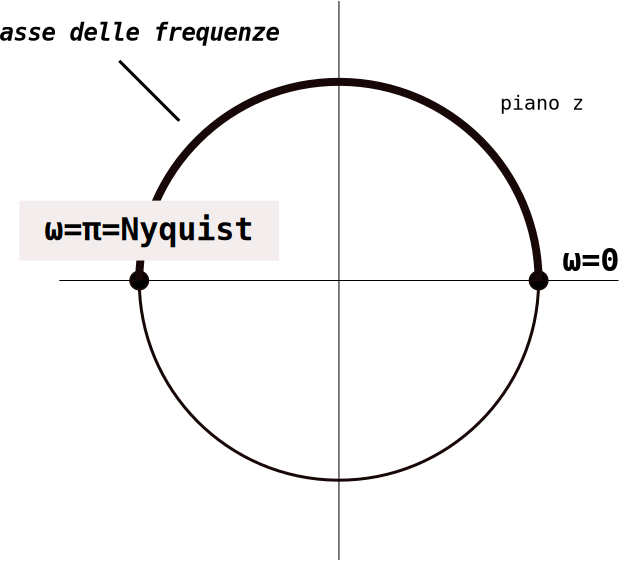
\includegraphics[width=0.4\textwidth]{\imagedir/frequency_axis_z_plane}
	\caption{L'asse delle frequenze sul piano $z$.\label{fig: z plane frequency axis}}
\end{center}
\end{figure}

Ora guardiamo pi\`u attentamente la funzione di trasferimento del nostro
esempio. Essa \`e

\begin{equation}\label{eq: simple transfer function 2}
				\mathpzc{H} ( z ) = 1 - a_1 z^{-1}
\end{equation}

Riscriviamola ora come rapporto di polinomi moltiplicando sopra e sotto per $z$:

\begin{equation}\label{eq: simple transfer function 3}
				\mathpzc{H} ( z ) = 1 - a_1 z^{-1} = \frac{z}{z} - \frac{a_1}{z} = \frac{z - a_1}{z}
\end{equation}

In questo modo appaiono chiaramente le radici dell'equazione:
c'\`e uno zero nel numeratore a $z = a_1$ e uno zero nel denominatore a $z = 0$. Vale a dire:
la funzione di trasferimento diventa zero a $z = a_1$ e infinita per $z = 0$.
La magnitudine della risposta in frequenza \`e la magnitudine di $\mathpzc{H} ( z )$
calcolata sul cerchio unitario (cio\`e quando $z = e^{i \omega}$):

\begin{equation}\label{eq: simple magnitude}
	| H ( \omega ) | = \frac{| z - a_1 |}{| z |}
\end{equation}

$| z | = 1$ perch\'e ci troviamo sul cerchio unitario (dato che $z = e^{i \omega}$).
In effetti, nei filtri \emph{feed-forward} (FIR) gli unici zeri al
denominatore possono apparire solo all'origine, e non hanno quindi alcun
effetto sulla risposta in frequenza. Possiamo quindi riscrivere l'Eq.\ref{eq: simple magnitude}
cos\`i:

\begin{equation}\label{eq: simple magnitude rewritten}
				| H ( \omega ) | = | z - a_1 |~\text{per}~z = e^{i \omega}
\end{equation}
\begin{figure}[htp]
\begin{center}
				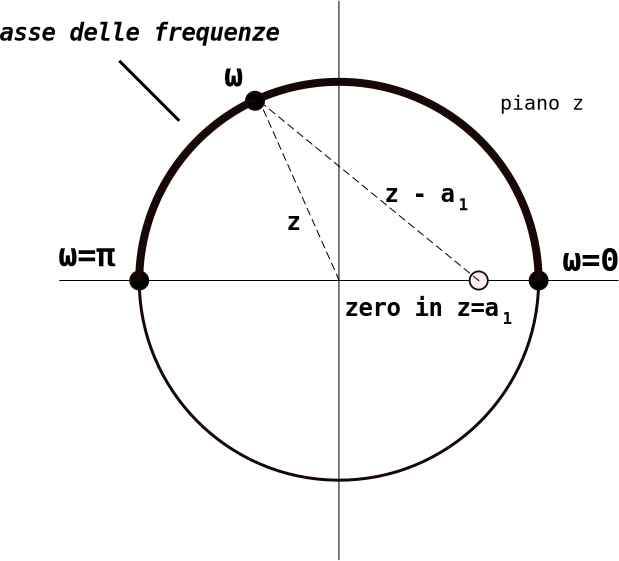
\includegraphics[width=0.4\textwidth]{\imagedir/mag_response}
				\caption{Valutazione della risposta in magnitudine per $z = e^{i
				\omega}$. Il fattore $|z - a_1|$ \`e la lunghezza del vettore dallo
				zero in $a_1$ sino al punto sul cerchio unitario corrispondente alla
				frequenza $\omega$\label{fig:mag response}}
\end{center}
\end{figure}

Ecco il significato della figura \ref{fig:mag response}: immaginiamo di
camminare sul cerchio unitario da $\omega = 0$ sino a $\omega = \pi$.
Quando ci troveremo vicino a $\omega = 0$, il modulo del vettore $|z - a_1|$
sar\`a molto piccolo e quindi influir\`aà molto sulla magnitudine del 
della funzione di trasferimento (riducendola). Man mano che ci allontaneremo
da $\omega = 0$ il modulo aumenter\`a e di conseguenza anche la magnitudine
della funzione di trasferimento. Quindi \`e ovvio che la Fig.\vref{fig:mag
response} ci sta mostrando la funzione di trasferimento di un filtro
passa--alto. Mentre per $a_1$ negativi si avrebbe un filtro passa--basso.
\begin{figure}[htp]
\begin{center}
				\includegraphics[width=0.85\textwidth]{\plotdir/zplane}
				\caption{La funzione $|\mathpzc{H}(z)|$ sul piano $z$\label{fig:mag response z plane}}
\end{center}
\end{figure}

La figura \vref{fig:mag response z plane} illustra la magnitudine della
funzione $z$ all'interno del cerchio unitario per $a_1 = 0.8$.


% completare la sezione


%
% $Id: z_transform.tex 14 2014-02-04 22:36:30Z nicb $
%

\svnInfo $Id: z_transform.tex 14 2014-02-04 22:36:30Z nicb $

\section{La trasformata \emph{zeta}}

\begin{itemize}

  \item funzioni di variabile complessa: come sono fatte?
    funzioni di mappatura tra un piano e un altro;
    esempi: $\frac{1}{z}$, $\frac{1}{z^2}$, ecc.

  \item trasformata $z$:
	
		 \begin{equation}
	      X ( z ) = \sum_{n = 0}{x(n) z^{-n}}\
		 \end{equation}
		 
    quando $z = e^{i \omega t}$ la trasformata z d\`a la risposta in freq.

  \item perch\'e si usa? perch\'e trasforma la sequenza di campioni in
    un polinomio, e un polinomio si pu\`o trattare matematicamente
    (== \`e possibile vedere cosa ``fa'' su tutto il piano z)

  \item radice di un polinomio $\Rightarrow$ quando il polinomio va a zero


\end{itemize}


%
% sezione sulla convoluzione
%

\section{L'operazione di convoluzione\label{sec:convolution}}

L'operazione di convoluzione \`e la somma di una sorta di moltplicazione
``scorrevole'' di un segnale con una data risposta all'impulso.
In pratica, questa operazione permette di analizzare il contributo della
moltiplicazione di ciascun campione del segnale
a un dato tempo $t$
con \emph{tutti} i campioni della risposta all'impulso.

Per esempio: il contributo della moltiplicazione della
risposta all'impulso $h_t$ con il campione $x_0$ al tempo $t$ sar\`a:

\begin{equation}
  x_0 h_t
\end{equation}

mentre quella del campione $t_1$ al tempo $t$ sar\`a:

\begin{equation}
  x_1 h_{t-1}
\end{equation}

ecc.

Quindi, tipicamente il contributo della moltiplicazione della risposta
all'impulso con il segnale $x_k$ \`e $x_k h_{t-k}$.

Dato che gestiamo sistemi lineari, possiamo sommare insieme tutti questi
contributi per avere il risultato finale:

\begin{equation}\label{eqn:generic convolution}
  y_t = \sum_{k = -\inf}^{\inf}{x_k h_{t-k}}
\end{equation}

Insomma, si tratta di un'operazione che permette di ricavare un terzo segnale
dalla moltiplicazione ``scorrevole'' di due segnali sommando poi insieme tutti
i contributi. Siccome si tratta di un'operazione molto usata, \`e stato
inventato un operatore e un simbolo apposta per lei:

\begin{equation}
  y = x \convolution h
\end{equation}

Nel caso dell'equazione \vref{eqn:generic convolution} i limiti della somma di
convoluzione sono tra $-\inf$ e $+\inf$, ma generalmente si tratta di
operazioni fatte su segnali finiti con risposte all'impulso finite. Usando ad
esempio segnali \emph{causali} che iniziano al tempo $t = 0$ e terminano entro
il tempo $t$, la convoluzione diventa semplicemente:

\begin{equation}
  y_t = \sum_{k = 0}^{t}{x_k h_{t-k}}
\end{equation}

Esercitiamoci ora con l'operazione di convoluzione, per capire esattamente
come funziona. Prendiamo un segnale di tre campioni $x = \{ 1, 2, 3 \}$ e una
risposta all'impulso $h = \{ 4, 5, 6 \}$. Ecco un modo intuitivo di ``vedere''
l'operazione di convoluzione:

\begin{equation}
  \begin{array}{*{5}{r} l}
  \multicolumn{6}{l}{al~tempo~t_{0}}\\
  1 & & & & & \times\\
  4 & 5 & 6 & & & =\\
  \hline
	4 & 5 & 6 & & & uscita~al~tempo~t_{0}\\
  \hline\hline
  \multicolumn{6}{l}{al~tempo~t_{1}}\\
  4 & 5 & 6 & & & +\\
    & 2 & & & & \times\\
    & 4 & 5 & 6 & & =\\
  \hline
  4 & 13 & 16 & 12 & & uscita~al~tempo~t_{1}\\
  \hline\hline
  \multicolumn{6}{l}{al~tempo~t_{2}}\\
  4 & 13 & 16 & 12 & &  +\\
  &  & 3  & & & \times\\
  &  & 4  & 5 & 6 & =\\
  \hline
  4 & 13 & 28 & 27 & 18 & uscita~al~tempo~t_{2}\\ 
\end{array}
\end{equation}

Dopo il tempo $t_2$ non ci sono pi\`u campioni non-zero, quindi il risultato
sar\`a sempre zero. Quindi:

\begin{equation}
  \{ 1, 2, 3 \} \convolution \{ 4, 5, 6 \} = \{ 4, 13, 28, 27, 18 \}
\end{equation}

Come si pu\`o notare, l'uscita dell'operazione di convoluzione \`e lunga $N + M - 1$,
dove $N$ \`e il numero dei campioni in ingresso e $M$ \`e il numero dei campioni della risposta all'impulso.

\paragraph{Esercizi}

\begin{compactenum}

  \item implementare ``a mano'' l'operazione di convoluzione in linguaggio {\tt matlab/octave} (costruire la funzione {\tt myconv}
        e verificarne il corretto funzionamento con la funzione {\tt conv}

  \item verificare le seguenti propriet\`a dell'operazione di convoluzione:
        commutativit\`a, associativit\`a, operazione neutra

  \item verificare il risultato della convoluzione di un segnale di lunghezza
        a piacere con una funzione gradino (nota come \emph{funzione di
        Heavyside}), e cio\`e con 
			  \begin{equation}	
				   h = \{ \ldots, 0, 0, 0, 1, 1, 1, 1, 1, 1, \ldots \}\nonumber
				\end{equation}
        Qual'\`e l'uscita che ci si attende?

\end{compactenum}

% TODO:
% subsection: la convoluzione di due segnali equivale alla moltiplicazione dei
%             loro spettri (fare rumore bianco per dente di sega rovesciato)
%
\subsection{Convoluzione e spettri}

La convoluzione di due segnali equivale alla moltiplicazione delle magnitudini
delle loro rappresentazioni in frequenza (spettri).

Facciamo il seguente esperimento:
prendiamo del rumore bianco (rappresentato nel dominio del tempo e nel dominio
della frequenza in Fig.\vref{fig:white noise}).

\begin{figure}[hbt]
  \begin{center}
	  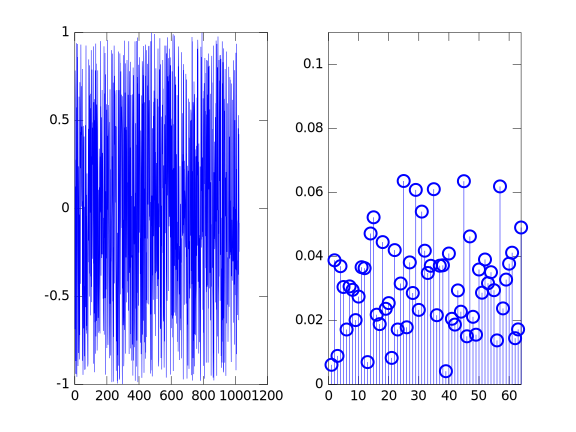
\includegraphics[width=0.8\textwidth]{\plotdir/conv_noise_and_saw_1}
   \end{center}
	\caption{Rumore bianco nel dominio del tempo e in quello della frequenza\label{fig:white noise}}
\end{figure}

Usiamo un'onda a dente di sega (rappresentata in Fig.\vref{fig:sawtooth}) come
risposta all'impulso.

\begin{figure}[hbt]
  \begin{center}
	  \includegraphics[width=0.8\textwidth]{\plotdir/conv_noise_and_saw_2}
  \end{center}
	\caption{Onda a dente di sega nel dominio del tempo e in quello della frequenza\label{fig:sawtooth}}
\end{figure}

Convolvendo il rumore bianco per l'onda a dente di sega otterremo la
moltiplicazione delle magnitudini delle due rappresentazioni spettali (cf.
Fig.\vref{fig:noise and saw convolved}),

\begin{figure}[hbt]
  \begin{center}
	  \includegraphics[width=0.8\textwidth]{\plotdir/conv_noise_and_saw_3}
  \end{center}
	\caption{Convoluzione dei due segnali\label{fig:noise and saw convolved}}
\end{figure}

Il codice {\tt matlab/octave} che produce questi grafici \`e riportato qui di
seguito:

\verbatiminput{\plotdir/conv_noise_and_saw.m}


\chapter{I filtri FIR\label{chap:fir}}

%
% $Id: FIR.tex 14 2014-02-04 22:36:30Z nicb $
%

\section{Un filtro FIR semplice\label{sec:simple fir}}

\subsection{Dominio continuo del tempo\label{sec:continuous time}}

Nei filtri FIR (\emph{feed-forward}) l'output \`e la somma dell'input e una versione riscalata e ritardata
		dell'input:

		\begin{equation}\label{eqn:fir semplice}
						y_t = x_t + a_1 x_{t-\tau}
			\end{equation}

		(aggiungere grafico)

	Poniamo che $x_t$ sia un segnale sinusoidale complesso:

		 \begin{equation}
	    x_t = e^{i\omega t}\nonumber
		 \end{equation}

		 \begin{equation}
			y_t = e^{i \omega t} + a_1 e^{i \omega (t - \tau)}
		 \end{equation}

		(fare schemino sul cerchio unitario)

		 \begin{equation}
		  y_t = e^{i \omega t} + a_1 e^{i \omega t} e^{-i \omega \tau} = e^{i\omega t} \left [ 1 + a_1 e^{-i \omega \tau} \right ]
		 \end{equation}

	Quindi l'uscita \`e sempre un fasore di frequenza $\omega$ moltiplicato per
		un'ampiezza che \`e funzione di $\omega$ (ma indipendente dal tempo!).

	La funzione del filtro \`e dunque $\left [ 1 + a_1 e^{-i \omega \tau} \right ]$ e la chiameremo $H(\omega)$

	Per capire la risposta in frequenza e in fase dobbiamo capire che $H(\omega)$ \`e
		in realt\`a la magnitudine (valore assoluto di $H(\omega)$ moltiplicata per una
		funzione della fase:

		 \begin{equation}
		  H(\omega) = |H(\omega)| e^{i \Theta(\omega)}
		 \end{equation}

	 dove $|H(\omega)| = |1 + a_1 e^{-i\omega \tau}|$; siccome per il teorema di Pitagora il
	 modulo \`e il quadrato della parte reale + il quadrato della parte
	 immaginaria sotto radice,

		 \begin{equation}
	  Re(H(\omega)) = 1 + a_1 cos(\omega \tau)
		 \end{equation}
		 \begin{equation}
		Im(H(\omega)) = - a_1 sin(\omega \tau)
		 \end{equation}

		 \begin{equation}
	  Re^2 = 1 + 2 a_1 cos(\omega \tau) + a_1^2 cos^2(\omega \tau)
		 \end{equation}
		 \begin{equation}
		Im^2 = a_1^2 sin^2(\omega \tau)
		 \end{equation}

		quindi
		
		 \begin{equation}
		Re^2 + Im^2 = 1 + 2 a_1 cos(\omega \tau) + a^2 [ cos^2(\omega \tau) + sin^2(\omega \tau) ]
		 \end{equation}

		 Dato che

		 \begin{equation}
				cos^2(\alpha) + sin^2(\alpha) = 1
		 \end{equation}

		 per $\alpha$ qualsiasi,

		 \begin{equation}
				1 + 2 a_1 cos(\omega \tau) + a^2 [ cos^2(\omega \tau) + sin^2(\omega \tau) ] = 1 + 2 a_1 cos(\omega \tau) + a^2
		 \end{equation}
		 \begin{figure}[htb]
			 \begin{center}
					\includegraphics[width=0.8\textwidth]{\plotdir/fir2}
					\caption{Filtro FIR con $\tau = 1/fc$\label{fig:fir con tau 1}}
			 \end{center}
		 \end{figure}
		 \begin{figure}[htb]
			 \begin{center}
					\includegraphics[width=0.8\textwidth]{\plotdir/fir3}
					\caption{Filtro FIR con $\tau = 23/fc$\label{fig:fir con tau 23}}
			 \end{center}
		 \end{figure}
		 Le Figg.\vref{fig:fir con tau 1} e \vref{fig:fir con tau 23} mostrano la
		 risposta in frequenza rispettivamente per $\tau = 1/fc$ e per $\tau = 23/fc$.

\paragraph{Esercizi}

\begin{itemize}

  \item fare il plot della risposta in frequenza con vari valori di $\omega$ e
          di $\tau$

\end{itemize}


\subsection{Passaggio dal tempo continuo al tempo discreto}


  Il ritardo $\tau$ viene ristretto ad un numero intero di campioni multiplo della
    periodo di campionamento $T_s$ (restrizione).

  Dato che la frequenza di campionamento interesser\`a  la  definizione
    del  nostro  segnale  (per  le  frequenze  che   servono   per   una
    applicazione piuttosto che un'altra), ma non  il  funzionamento  del
    filtro, possiamo  benissimo  normalizzare  la  nostra  frequenza  di
    campionamento a $1$, avendo cos\`i la frequenza di Nyquist a $0.5$.

  Ora, se noi ritardiamo il nostro segnale di un campione (invece che del
    valore continuo tau) moltiplicheremo il nostro fasore in ingresso per
    $e^{-i \omega T}$ dove $\omega T$ \`e l'angolo in radianti per campione. Possiamo sempre
    ricavare il tempo nel dominio digitale moltiplicando per il periodo di
    campionamento $T_s$ - possiamo quindi evitare di scrivere $T_s$, che diventa
    una sorta di costante di conversione: se la costante \`e 1 (frq di
    campionamento 1) possiamo evitare di scriverla ogni volta.

  La frequenza di campionamento diventa $\omega = 2 \pi$ e la frequenza di nyquist \`e
    $\omega = \pi$ radianti per campione e il nostro fasore sar\`a sempre

     \begin{equation}
        x_t = e^{i\omega kT}
     \end{equation}
    
    dove $k$ \`e un numero intero di campioni e $T$ \`e il periodo di campionamento.

    Ora rifacciamo il filtro dell'eq.\ref{eqn:fir semplice} della Sez.\vref{sec:continuous time} ritardando per\`o non di tau
    ma di un solo campione:

     \begin{equation}
       y_k = x_k + a_1 x_{k-1}
     \end{equation}

    applicando il fasore digitale, il filtro diventer\`a:

     \begin{equation}
        y_k = e^{i\omega kT} [ 1 + a_1 e^{-i\omega \times 1} ] = e^{i \omega kT} [ 1 + a_1 e^{-i \omega } ]
     \end{equation}

    e la magnitudine (== risposta in frequenza) sar\`a:

     \begin{equation}
       |H( \omega )| = \sqrt{1 + 2 a_1 cos( \omega ) + a_1^2}
     \end{equation}

  Ricapitolando, se l'input di un filtro FIR \`e il fasore $e^{i \omega kT}$

     \begin{equation}
     y_t = a_0 x_t + a_1 x_{t-1}
     \end{equation}

    (ritardo di un campione).

    L'output \`e anche un fasore con frequenze inalterate

     \begin{equation}
     y_k = x_k \left [ a_0 + a_1 e^{-i \omega} \right ]
     \end{equation}

    possiamo aggiungere quanti termini vogliamo in un filtro del genere:

     \begin{equation}
     y_k = x_k \left [ a_0 + a_1 e^{-i\omega } + a_2 e^{-i2\omega } + a_3 e^{-i3\omega } + ... + a_n e^{-in\omega } \right ]
     \end{equation}


  Invece di ripetere $e^{i\omega}$ ogni volta, possiamo operare una sostituzione: sostituiamo $z = e^{i \omega}$

  Il ritardo di un campione diventa cos\`i $z^{-1}$, e il ritardo di $k$ campioni
    diventa cos\`i $z^{-k}$

  $z^{-1}$ \`e trattabile sia come una variabile complessa che come un
    operatore, cio\`e una operazione applicata ad un certo oggetto (pensate
    p.es. ad un operatore che ruota un disegno di 90 gradi) $= \rho$: $\rho^2$ lo
    ruota di 180 gradi in senso antiorario, $\rho^{-1}$ lo ruota in senso orario).

  Possiamo anche usare la notazione $X$ per rappresentare un \emph{intero segnale}
    (un vettore di campioni); nota bene: $x_k$ rappresenta il valore di un
    segnale al tempo $k$, $X$ rappresenta \emph{l'intero segnale}.

  L'intero segnale ritardato di un campione \`e quindi notato $z^{-1} X$ quindi
    significa ``applica l'operatore $z^{-1}$ al segnale $X$''

    L'equazione si riscrive:

     \begin{equation}
      Y = a_0 X + a_1 z^{-1} X = \left [ a_0 + a_1 z^{-1} \right ] X
     \end{equation}

    (nota che anche l'ampiezza diventa un operatore: moltiplica \emph{tutto il
    segnale} per la costante $a_0$, e quest'operatore \`e commutativo).

  Quindi $Y = H(z) X$ dove $H(z) = a_0 + a_1 z^{-1}$.

% \item se del caso fare due filtri in cascata moltiplicando le funzioni di
%   trasferimento

\paragraph{Esercizi}

\begin{enumerate}

  \item Si descriva un filtro FIR con l'equazione che segue:

          \begin{equation}
            y_k = x_k + x_{k-1} + x_{k-2} + \ldots + x_{k-19}
          \end{equation}

        Si derivi una espressione algebrica semplice per la sua risposta in
        magnitudine. Si trovi quali siano le frequenze alle quali si trovano
        dei picchi e quelle alle quali si trovano dei buchi

\end{enumerate}


%
% $Id: ripasso_FIR.tex 14 2014-02-04 22:36:30Z nicb $
%
\svnInfo $Id: ripasso_FIR.tex 14 2014-02-04 22:36:30Z nicb $

\section{Trasformata zeta applicata ai filtri FIR\label{sec:zeta fir}}

\subsection{Ritardo e linearit\`a\label{sec:ritardo e linearita}}

Recuperiamo le propriet\`a della trasformata Z e applichiamole ai filtri FIR.

\begin{itemize}

\item filtro FIR:
				
		\begin{equation}
			X(k)\,\raiseto{H}\,Y(k)
		\end{equation}

		La forma generalizzata di un filtro FIR \`e:
  
		\begin{equation}
    	Y(k) = C(1)X(k) + C(2)X(k-1) + ... + C(M)X(k-M+1)
		\end{equation}

\item per via della propriet\`a 2 della trasformata Z (linearit\`a) la trasformata Z di questa somma
     \`e uguale alla somma delle trasformata Z di ogni termine. Per via della propriet\`a
     1, ciascun termine pu\`o essere letto come multiplo della trasformata Z di $X(k)$,
     perch\'e:
 
		 \begin{equation}
			 \begin{array}{r c l}
						 C(1)X(k) & \raiseto{Z} & C(1)X^{*}(z)\\
						 C(2)X(k-1) & \raiseto{Z} & C(2)z^{-1}X^{*}(z)\\
						 C(3)X(k-2) & \raiseto{Z} & C(3)z^{-2}X^{*}(z)\\
						            & \vdots & \\
						 C(M)X(k-M+1) & \raiseto{Z} & C(M)z^{(-M+1)}X^{*}(z)\\
		    \end{array}
		 \end{equation}
 
     quindi:

		 \begin{equation}
						 Y(k)\,\raiseto{Z}\,Y^{*}(z) = [ C(1)+C(2)z^{-1}+C(2)z^{-2}+ \ldots +C(M)z^{-(M+1)} ] X^{*}(z)
		 \end{equation}
 
		 ponendo
 
		 \begin{equation}
			 H(z) = [ C(1)+C(2)z^{-1}+C(2)z^{-2}+ \ldots +C(M)z^{-(M+1)} ]
		 \end{equation}
 
     ossia
 
		 \begin{equation}
						 H(z) = \frac{Y^{*}(z)}{X^{*}(z)}
		 \end{equation}
 
\item quindi: quando $X$ \`e un fasore, anche $Y$ \`e un fasore e il rapporto tra $X$ e
			$Y$ \`e proprio $H(z)$ (quando $z = e^{i\omega}$): quando io metto dentro al filtro un
      segnale sinusoidale ottengo un segnale sinusoidale riscalato

\item ma la faccenda \`e molto pi\`u generale: quando X  \`e  un  qualsiasi
      segnale causale (one-sided), l'uscita di un black box pu\`o  essere
      ottenuta semplicemente moltiplicando la sua trasformata $Z$  per  la
      funzione di trasferimento $H(z)$
 
			\begin{itemize}

			\item facciamo un esempio semplice:
 
				\begin{equation}
	 			\begin{array}{c c c l}
	  			X(k) & = & 0  & \quad per~k~<~0\\
         X(0) & = & 1  &          \\
         X(1) & = & 1  &          \\
				 X(k) & = & 0  & \quad per~k~>~1\\
					\end{array}
			 \end{equation}
 
 \item dalla definizione di trasformata Z ($X^{*}(z) = \sum_0^{N}{X(n)z^{-n}}$), la trasformata di questo segnale \`e:

				 \begin{equation}
								 X^{*}(z) = 1 + z^{-1}
				 \end{equation}
 
 \item ora filtriamolo col solito filtro di media semplicissimo:
 
		 		\begin{equation}
        	 Y(k) = X(k) + X(k-1)
		    \end{equation}
 
 \item la funzione di trasferimento \`e:
 
		 \begin{equation}
						 H(z) = 1 + z^{-1}
		 \end{equation}
 
 \item quindi:
 
		 \begin{equation}
						 Y^{*}(z) = H(z)X^{*}(z) = (1+z^{-1})(1+z^{-1}) = 1 + 2 z^{-1} + z^{-2}
		 \end{equation}

 \item \`e facile fare la trasformata inversa perch\'e ci sono tutte potenze decrescenti
       di zeta, quindi:
 
			 	\begin{equation}
								\begin{array}{c c c l}
           Y(k) & = & 0 & per\,k\,<\,0 \\
           Y(0) & = & 1 & \\
           Y(1) & = & 2 & \\
           Y(2) & = & 1 & \\
           Y(k) & = & 0 & per\,k\,>\,2\\
								\end{array}
		 \end{equation}
 
       si pu\`o verificare la correttezza facendo girare ``a mano'' il filtro

			\end{itemize}
%
%    - dimostrare che la trasformata Z \`e unica per ogni segnale, cio\`e che se due
%      segnali hanno la stessa trasformata Z, allora sono identici
%

\end{itemize}

\paragraph{Esercizi}

\begin{itemize}
 
 \item rifare il filtraggio sopra esposto con il seguente segnale:

				 \begin{equation}
						X(x) = \left\{
						   \begin{array}{c l}
									1 & 0 <= k <= 10 (o\,\,anche\,<=\,5)\\
									0 & altrimenti\\
							 \end{array} \right.
		     \end{equation}
 
       e con le seguenti funzioni di trasferimento:
 
			 	\begin{equation}
					\begin{array}{c c c c c}
	  				H(z) & = & 1 & - & z^{-1}\\
						 H(z) & = & 1 & + & z^{-1}\\
             H(z) & = & ( 1 & - & z^{-1} )^2\\
	      	 \end{array}
	       \end{equation}

\end{itemize}

\section{Una collezione di trasformate zeta notevoli\label{sec:zeta notevoli}}

\subsection{La trasformata zeta pi\`u semplice}

		La trasformata pi\`u semplice \`e quella che prevede campioni  non  zero  per  un
     numero finito di campioni. Per come abbiamo visto l'altra volta, la
     trasformata  $Z$  di  un  segnale  del  genere  \`e  semplicemente  un
     polinomio in $z^{-1}$. P.es.:

		 \begin{equation}
				X(k) = \left\{
					\begin{array}{c c c c}
						0 & k & <= & 0\\
						.5 & k & = & 1\\
						1 & k & = & 2\\
						.5 & k & = & 3\\
						0 & k & > & 3\\
		\end{array} \right.
		 \end{equation}

     Per la definizione di trasformata Z, la trasformata Z di questo segnale \`e

		 \begin{equation}
	   	 X^{*}(z) = .5z^{-1} + z^{-2} + .5z^{-3}
		 \end{equation}

     E la trasformata inversa \`e semplicemente la sequenza dei coefficienti del
     polinomio (== come se fossero ciascuno moltiplicato per 1)

\subsection{Un caso pi\`u interessante}

Un caso pi\`u interessante ha luogo quando il segnale \`e non  zero  per
    un infinito/indefinito numero  di  valori  di  k,  cio\`e  quando  il
    segnale va avanti per sempre. Questo a noi fa comodo per i segnali audio.
    Per noi p.es. sono molto importanti classi di segnali che sono
    esponenziali o sinusoidali di natura, e one-sided.

    Il segnale pi\`u semplice \`e la unit-step function in cui $X(k) = 1$ per $k >= 0$.
		La sua trasformata $z$ \`e:

		 \begin{equation}
						 X^{*}(z) = 1 + z^{-1} + z^{-2} + z^{-3} + \ldots
		 \end{equation}

    Questa \`e una serie geometrica ben conosciuta e sappiamo dall'algebra che
    la sua trasformata $z$ \`e quindi:

		 \begin{equation}
			 X^{*}(z) = \frac{1}{1-z^{-1}}
		 \end{equation}

   La serie geometrica funziona cos\`i: poniamo una serie

		 \begin{equation}
			a + ar + ar^{2} + ar^{3} + ... + ar^{n-1} = \sum_{k=0}^{n-1}{ar^{k}} =  \left\{ a\frac{1-r^{n}}{1 - r} \right\}
		 \end{equation}

   come ci si arriva? poniamo:

		 \begin{equation}
    s = a + ar + ar^{2} + \ldots + ar^{n-1}
		 \end{equation}

   allora 

		 \begin{equation}
    sr = ar + ar^{2} + ar^{3} + ... + ar^{n}
		 \end{equation}

   ma $s - sr = a - ar^{n}$, quindi $s(1 - r) = a(1 - r^{n})$, quindi

		 \begin{equation}
				s = a \frac{1 - r^{n}}{1 - r}
		 \end{equation}

   quando $n$ va all'infinito, \`e necessario che $r < 1$ per far convergere la somma. In questo caso

	 $\sum_{k=0}^{\inf}{ar^{k}}$ diventa $=\frac{a}{1 - r}$ e se $a = 1$, $= \frac{1}{1 - r}$

   quindi 

		 \begin{equation}
			  X^{*}(z) = \frac{1}{1-z^{-1}}
		 \end{equation}

   a patto che $|z^{-1}| < 1$ e dato che $|z^{-1}| = \frac{1}{|z|}$ questo equivale a dire che $|z| > 1$

   Se esaminiamo questo polinomio pi\`u da vicino, e moltiplichiamo num e den
   per $z$, questo diventa:

		 \begin{equation}
						 \frac{z}{z - 1}
		 \end{equation}

   e per $z = 1$, la trasformata zeta diventa infinita. Questo punto si chiama
	 un \emph{polo}. In questo caso quindi la trasformata $z$ ha uno zero per $z = 0$ e
	 un polo per $z = 1$. (un piano con uno zero al centro e un polo sul 1 reale -- cf.Fig.\vref{fig:poli e zeri}).
	 \begin{figure}[Hbtp]
			\begin{center}
				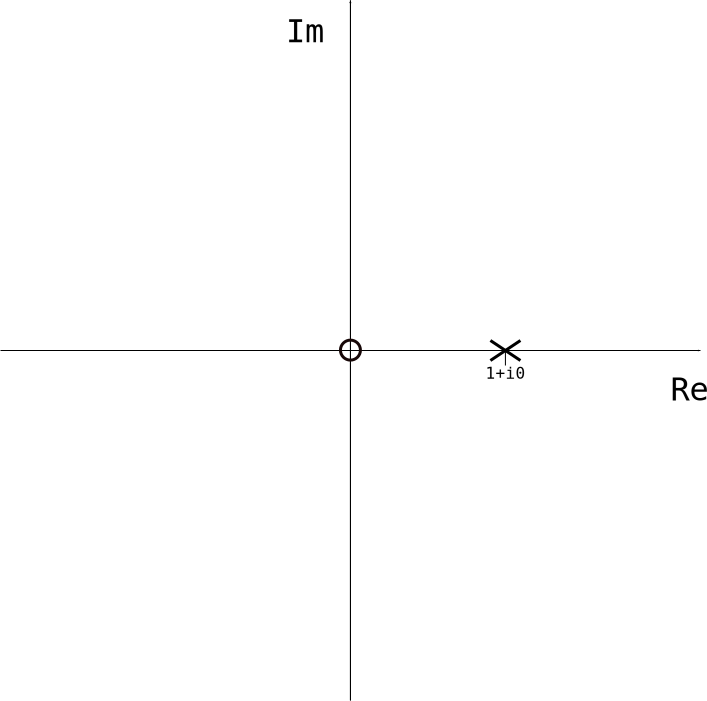
\includegraphics[width=0.35\textwidth]{\imagedir/piano_zeta_un_polo}
				\caption{Poli e zeri del filtro $X^{*}(z) = \frac{1}{1-z^{-1}}$\label{fig:poli e zeri}}
			\end{center}
	 \end{figure}
   Quindi a frequenza zero si sommano tutti gli uni e la somma infinita
   esplode. Possiamo trovare la magnitudine della trasformata $z$ sul cerchio
   unitario e questa si chiama ``contenuto frequenziale'' o \emph{risposta in
	 frequenza} del segnale. Ponendo $z = e^{-i\omega}$

		 \begin{equation}
				X^{*}(z) = \frac{1}{1 - e^{i\omega}}
		 \end{equation}

   la magnitudine (il modulo) \`e quindi:

		 \begin{equation}
				|X^{*}(z)| = \frac{1}{|1 - e^{i\omega}|}
		 \end{equation}


   e se moltiplico entrambi i membri del denominatore per $e^{-iw/2}$ ottengo

		 \begin{equation}
				 |X^{*}(z)| = \frac{1}{|e^{-i\omega/2} - e^{i\omega/2}|}
		 \end{equation}

   e quindi per via della formula di Eulero                 

	   \begin{equation}\label{eqn:infinitefir}
				 |X^{*}(z)| = \frac{1}{2 |sin {\omega/2}|}
		 \end{equation}
	\begin{figure}[htbp]	
		\begin{center}
			\includegraphics[width=0.4\textwidth]{\plotdir/infinitefir}
			\caption{Magnitudine dell'eq.\ref{eqn:infinitefir} con freq.  normalizzata}
		\end{center}
	\end{figure}


%
% $Id: fase.tex 14 2014-02-04 22:36:30Z nicb $
%
% p.76 cap.4 n.7
%
\svnInfo $Id: fase.tex 14 2014-02-04 22:36:30Z nicb $

\section{La risposta in fase\label{sec:phase}}

Riconsideriamo ancora una volta il filtro che abbiamo analizzato in
Cap.\ref{chap:fir} Sez.\vref{sec:simple fir} (eq.\ref{eqn:fir semplice}):

		\begin{equation}\label{eqn:fir semplice 2}
						y_t = x_t + a_1 x_{t-\tau}
			\end{equation}

la cui risposta in frequenza \`e una funzione della frequenza $\omega$

	\begin{equation}\label{eqn:fir semplice frqresp}
	       H ( \omega ) = 1 + a_1 e^{-i \omega}
	\end{equation}

Questa risposta complessa in frequenza avr\`a quindi una magnitudine e un
angolo per ciascun $\omega$. Cio\`e l'eq.\ref{eqn:fir semplice frqresp} pu\`o
essere riscritta come 

	\begin{equation}\label{eqn:fir semplice frqresp 2}
	       1 + a_1 e^{-i \omega} = |H ( \omega )| e^{i \Theta ( \omega )}
	\end{equation}

Se il segnale in ingresso fosse un fasore complesso $x = e^{i \omega t}$,
il fasore in uscita $y$ sarebbe il prodotto di questo ingresso moltiplicato
questa funzione di trasferimento

	\begin{equation}\label{eqn:fs output}
		y_t = |H ( \omega )|e^{i (\omega t + \Theta ( \omega ) )}
	\end{equation}

il che significa che l'uscita \`e una copia dell'ingresso ritardata in fase di
un angolo $\Theta ( \omega )$ e riscalata in ampiezza di $| H ( \omega )|$.

Per capire quanto valga il ritardo di fase possiamo usare la funzione
\emph{arcotangente}. Riscrivendo l'eq.\ref{eqn:fir semplice frqresp} come $1 +
a_1 cos \omega - i a_1 sin \omega$, avremo

  \begin{equation}\label{eqn:risp in fase}
			\begin{array}{r c l}
							\Theta ( \omega ) & = & arctan \left [ \frac{\mathpzc{Immag} H ( \omega )}{\mathpzc{Reale} H ( \omega )} \right ]\\
							                  & = & arctan \left [ \frac{- a_1 sin \omega}{1 + a_1 cos \omega} \right ]\\
			\end{array}
	\end{equation}

Quando $a_1 = 1$ l'espressione contenuta in eq.\ref{eqn:risp in fase} si
semplifica. Riscrivendo la funzione di trasferimento di eq.\ref{eqn:fir semplice frqresp}
con $a_1 = 1$:

	\begin{equation}\label{eqn:fir semplice frqresp 3}
			H ( \omega ) = 1 + e^{-i \omega} = e^{-i \omega / 2} \left [ e^{i \omega / 2} + e^{-i \omega / 2} \right ]
	\end{equation}

Ricordiamo che la formula di Eulero $e^{i \alpha} = cos \alpha + i sin
\alpha$, e che quindi

	\begin{equation}\label{eqn:remember eulero}
			\begin{array}{r c l}
							cos \alpha & = & \frac{e^{i \alpha} + e^{-i \alpha}}{2}\\
							sin \alpha & = & \frac{e^{i \alpha} - e^{-i \alpha}}{2i}\\
							e^{i \alpha} + e^{-i \alpha} & = & 2 cos \alpha\\
							e^{i \omega / 2 } + e^{-i \omega / 2} & = & 2 cos \omega / 2\\
			\end{array}
	\end{equation}

	allora l'eq.\ref{eqn:fir semplice frqresp 3} si semplifica in

  \begin{equation}\label{eqn:fir semplice frqresp 3 result}
		H (\omega) =  e^{-i \omega / 2} 2 cos (\omega / 2)\\
	\end{equation}

Confrontando l'eq.\ref{eqn:fir semplice frqresp 2} con la \ref{eqn:fir semplice frqresp 3 result},
$2 cos (\omega / 2)$ \`e la magnitudine della risposta (reale) $|H ( \omega )|$,
mentre l'esponenziale complesso $e^{-i \omega / 2}$ \`e la risposta in fase
e rappresenta un ritardo di fase di un angolo $- \omega / 2$.
Quindi, se l'ingresso \`e il fasore $e^{i \omega t}$, l'uscita del filtro
sar\`a il fasore

	\begin{equation}\label{eqn:fir output}
			2 cos ( \omega / 2 ) e^{i \omega (t - 1 / 2)}
	\end{equation}

il che equivale a dire che l'effetto del filtro sulla fase del segnale \`e
quello di ritardarlo esattamente di un tempo equivalente alla met\`a della
frequenza di campionamento, \emph{indipendentemente dalla frequenza} $\omega$
\emph{del fasore in ingresso}.

Questo \`e un caso speciale di una caratteristica importante dei filtri FIR:
se i coefficienti di un filtro FIR sono simmetrici intorno al proprio centro
(in questo caso i coefficienti sono $\{ 1, 1 \}$, la risposta in fase \`e
proporzionale ad $\omega$, trattandosi quindi di un ritardo di tempo fisso per
tutte le frequenze. Il filtro si dice quindi \emph{a fase lineare}, ossia non
introduce distorsioni nella risposta in fase.

La fig.\vref{fig: fase 3} riporta la risposta in frequenza e la risposta in
fase del filtro FIR

\begin{equation}\label{eqn: fir 3}
	H ( z ) = 0.5 - 0.8 z^{-1} + 0.5 z^{-2}
\end{equation}
\begin{figure}[htb]
	\begin{center}
	\includegraphics[width=0.9\textwidth]{\plotdir/fase_3}
	\caption{Risposta in frequenza e in fase del filtro la cui funzione di
	trasferimento \`e riportata in eq.\ref{eqn: fir 3}\label{fig: fase 3}}
	\end{center}
\end{figure}

Come si pu\`o notare, un numero dispari di coefficienti genera una risposta in
fase lineare.

Lo script {\tt octave} che genera questa figura \`e riportato qui:

\verbatiminput{\plotdir/fase_3.m}


%
% $Id: icf.tex 14 2014-02-04 22:36:30Z nicb $
%
% p.77 cap.4 n.8
%
\svnInfo $Id: icf.tex 14 2014-02-04 22:36:30Z nicb $

\section{Introduzione\label{sec:icf introduction}}

I filtri comb inversi sono un caso particolare di filtri FIR. Essi permettono,
ad esempio, di cancellare le componenti di un segnale armonico.

Si tratta come sempre di un filtro FIR come quello studiato in
Sez.\ref{sec:simple fir}.\vref{sec:continuous time}  (eq.\ref{eqn:fir
semplice}). Sostituiamo al posto del ritardo arbitrario $\tau$ un numero
intero di campioni $L$. Come coefficiente del filtro prenderemo $R^{L}$.

L'equazione diventer\`a quindi

\begin{equation}\label{eqn:icf 1}
		y_t = x_t - R^{L} x_{t - L}
\end{equation}

e la sua funzione di trasferimento si ricaver\`a cos\`i

\begin{equation}\label{eqn: icf 1 tf}
  \begin{array}{r c l c c l}
	Y & = & 1 \times X z^{-0} - R^{L} \times X z^{-L} & = & X & \left [ 1 - R^{L} z^{-L} \right ]\\ 
	H ( z ) & = &                                     &   &   & \left [ 1 - R^{L} z^{-L} \right ]\\
	\end{array}
\end{equation}

\begin{quote}
Ripassiamo un p\`o di algebra dei numeri complessi.
Quali sono le radici dell'equazione seguente:

\begin{equation}\label{eqn: icf roots}
      z^{L} = 1
\end{equation}

Il teorema fondamentale dell'algebra dice che un polinomio di grado $n$ ha $n$
radici ($n$ punti in cui la funzione \`e zero). Prendiamo ad es.

\begin{equation}\label{eqn: tfa 1}
		y = x^{2} - 9
\end{equation}

Dobbiamo trovare i punti in cui $y = 0$. Allora:

\begin{equation}\label{eqn: tfa 2}
	\begin{array}{r c l}
		x^{2} - 9 & = & 0\\
		x^{2}     & = & 9\\
		x         & = & \sqrt{9}\\
		x         & = & \pm 3\\
	\end{array}
\end{equation}

% fare plot della funzione

E` possibile quindi pensare qualsiasi funzione nei termini delle sue radici:

\begin{equation}\label{eqn: tfa 3}
		y = a_1 ( x - r_1 ) (x - r_2) \dots
\end{equation}

P.es. nel caso dell'eq.\ref{eqn: tfa 2}

\begin{equation}\label{eqn: tfa 4}
	x^{2} - 9 = 1 ( x + 3 ) ( x - 3 )
\end{equation}

Spesso \`e necessario ricorrere ai numeri complessi per risolvere le
equazioni. P.es., quali sono le radici dell'eq.\ref{eqn: tfa complex 1}?

\begin{equation}\label{eqn: tfa complex 1}
	x^2 - x + 1 = 0
\end{equation}

Ricordando che

\begin{equation}\label{eqn: tfa complex 2}
				x = \frac{-b \pm \sqrt{b^{2} - 4 a c}}{2 a}
\end{equation}

e sostituendo i fattori $a$, $b$, e $c$ con quelli presenti nell'eq.\ref{eqn: tfa complex 1}

\begin{equation}\label{eqn: tfa complex 3}
				x = \frac{+1 \pm \sqrt{-1^{2} - 4 \times 1 \times 1}}{2 \times 1} = \frac{\pm \sqrt{1 - 4}}{2} = \frac{1}{2} \pm i \frac{\sqrt{3}}{2} = 0.5 \pm i 0.866
\end{equation}

In linea generale, le equazioni di grado $n$ con fattori complessi possiedono
$n$ radici in coppie complesse coniugate (per $n$ pari) oppure 1 radice reale
e $n - 1$ radici in coppie complesse coniugate (per $n$ dispari).
\end{quote}

Ecco dunque la risposta alla domanda: quali sono le radici dell'equazione $z^{L} = 1$?
ce ne sono $L$, complesse--coniugate e equispaziate sul cerchio
unitario. Questo \`e abbastanza ovvio quando si pensa a cosa significhi
innalzare un numero complesso alla sua $L$--esima potenza. Significa
elevare la sua magnitudine ($==$ il suo modulo) all'$L$--esima potenza e
moltiplicare il suo angolo per $L$. Qualsiasi punto con magnitudine 1 e
angolo in una forma $k 2 \pi / L$ funzioner\`a per qualsiasi $k$ intero.
Le $L$ radici dell'unit\`a saranno quindi:

\begin{equation}\label{eqn: roots of unity}
		e^{i k 2 \pi / L}~per~k = 0, 1, \dots, L - 1
\end{equation}

E nel caso dell'eq.\ref{eqn: icf 1 tf} le radici saranno:

\begin{equation}\label{eqn: roots of R}
		z^{L} = R^{L}
\end{equation}

e si troveranno agli stessi angoli, ma con raggio $R^{L}$ anzich\'e 1.

Facciamo un esempio con $L = 8$ (cio\`e: il segnale sar\`a composto
dall'ingresso pi\`u l'ingresso ritardato di otto campioni) con $R = 0.999999$.

Ci aspetteremo quindi di trovare otto zeri, e per la precisione (dato che il
segnale finale \`e reale) quattro coppie complesse coniugate.
In effetti, il plot sul piano zeta rappresentato in Fig.\vref{fig: icomb 8 zeroes}
mostra proprio che gli otto zeri si dispongono in maniera simmetrica intorno
all'asse reale (e anche simmetrica intorno all'asse immaginario).

\begin{figure}[htbp]
	\begin{center}
		\includegraphics[width=0.48\textwidth]{\plotdir/ICF2_2}
	  \includegraphics[width=0.48\textwidth]{\plotdir/ICF2_3}
		\caption{Disposizione degli zeri sul piano zeta per un filtro comb inverso di ordine 8\label{fig: icomb 8 zeroes}}
	\end{center}
\end{figure}

Come si pu\`o notare, gli zeri appaiono a $R^{L} e^{i 2 pi \times 0/L} = 1$,
$R^{L} e^{i 2 \pi \times 1/L} = R^{L} e^{i 2 \pi / 8} = R^{L} e^{i \pi / 4} = 0.707 + i 0.707$,
$R^{L} e^{i 2 \pi \times 2 /L} = R^{L} e^{i 4 \pi / 8} = e^{i \pi /2} = i$, ecc.
La Fig.\vref{fig: icomb 8 bode} invece mostra che la fase \`e per lo pi\`u
lineare, con gli shift di fase che accadono al passaggio dagli zeri della
magnitudine.

\begin{figure}[htbp]
	\begin{center}
	  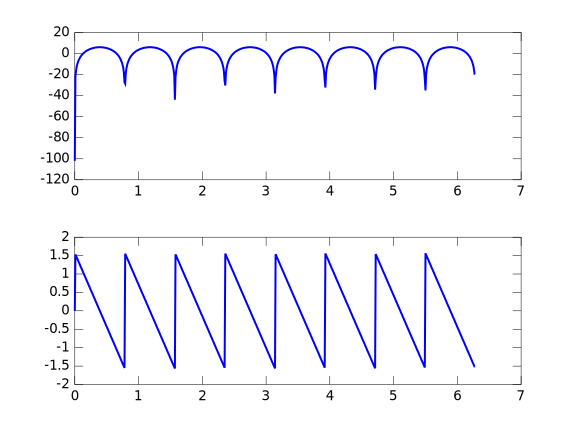
\includegraphics[width=0.8\textwidth]{\plotdir/ICF2_1}
	  \caption{Risposta in frequenza e in fase di un filtro comb inverso di ordine 8\label{fig: icomb 8 bode}}
	\end{center}
\end{figure}

\needspace{20\baselineskip}
Lo script \emph{octave} che produce questi plot \`e riportato qui di seguito:
\verbatiminput{\plotdir/ICF2.m}

Attenzione: un errore comune \`e quello di invertire l'ordine dei coefficienti nel
passare l'argomento alla funzione {\tt roots()} di \emph{matlab/octave}.
L'ordine \`e \ul{dal coefficiente pi\`u alto a quello pi\`u basso} (zero
incluso).

% esempio di signal cancellation
 % inverse comb filters

%
% $Id: filter_design.tex 14 2014-02-04 22:36:30Z nicb $
%
% cap.12
%
\svnInfo $Id: filter_design.tex 14 2014-02-04 22:36:30Z nicb $

\section{Introduzione alla progettazione di filtri FIR\label{sec: filter design introduction}}
%
% tecniche di design: ottimizzazione iterativa
%                   forme chiuse
%

Il problema sostanziale nel progettare i filtri \`e quello di trovare i giusti
coefficienti per raggiungere la migliore approssimazione alla ``risposta ideale''
che si desidera ottenere. In linea generale, la ``risposta ideale'' non \`e
ottenibile direttamente perch\'e si tratta di una funzione discontinua (che
non \`e realizzabile con un polinomio. Il problema \`e rappresentato in
fig.\vref{fig:ideal vs real}.
\begin{figure}[htbp]
	\begin{center}
		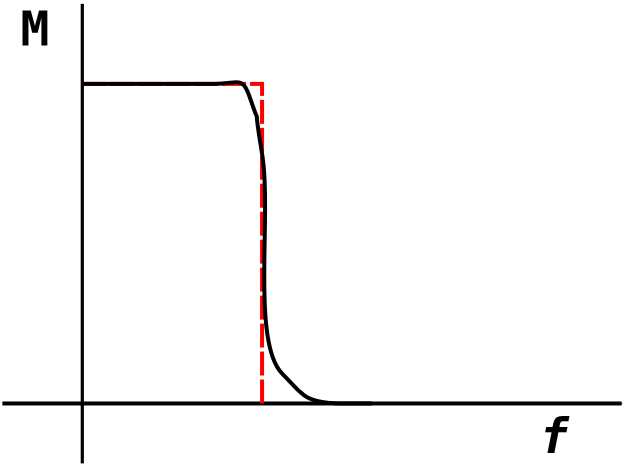
\includegraphics[width=0.75\textwidth]{\imagedir/ideal_vs_real}
		\caption{La risposta ideale di un filtro (in rosso) e la sua risposta reale\label{fig:ideal vs real}}
	\end{center}
\end{figure}

Ci sono varie soluzioni per ottenere questi coefficienti, e queste soluzioni
si applicano meglio a certi tipi di filtri che ad altri.
In alcuni casi \`e possibile (o necessario) trovare delle ``forme chiuse''
(vale a dire delle equazioni matematiche finite) per individuare i
coefficienti, mentre in altri casi \`e possibile trovarli attraverso una
``ottimizzazione iterativa'' (vale a dire ottenendo prima una approssimazione
mediocre per poi migliorarla a discrezione).

I coefficienti dei filtri FIR si trovano pi\`u facilmente attraverso
quest'ultima tecnica (ottimizzazione iterativa).

%
% ordine del filtro e simmetria dei coefficienti (0, N-1 per N coefficienti, N-1 ordine)
%

Ricordiamo che la forma dei filtri FIR \`e specificata da un'equazione del
tipo:

\begin{equation}
	y_t = a_0 x_t + a_1 x_{t-1} + a_2 x_{t-2} + \dots + a_{n-1} x_{t-(n-1)}
\end{equation}

Il primo coefficiente \`e il coefficiente $0$, quindi l'ultimo coefficiente di
un filtro di lunghezza $n$ \`e $n-1$. La sua funzione di trasferimento \`e

\begin{equation}
	H(z) = a_0 + a_1 z^{-1} + a_2 z^{-2} + \dots + a_{n-1} z^{-(n-1)}
\end{equation}

Considerando che la risposta $y_t$ deve essere una risposta reale, possiamo
semplificare la nostra progettazione utilizzando un numero pari di
coefficienti. Questi coefficienti distribuiranno gli zeri sul piano zeta in
posizioni complesse--coniugate ed il risultato sar\`a quindi reale.
Il problema \`e che abbiamo un coefficiente $0$, e che quindi se usiamo filtri
di lunghezza pari avremo una asimmetria intorno all'asse dei numeri reali.
Dobbiamo quindi utilizzare una lunghezza \emph{dispari} per ottenere un numero
\emph{pari} di coefficienti simmetrici (e un coefficiente direttamente
sull'asse reale -- che quindi sar\`a un numero reale).

Ad esempio, se usiamo un filtro di lunghezza 5, avremo la funzione di
trasferimento

\begin{equation}\label{eqn: fir order five}
		H(z) = a_0 + a_1 z^{-1} + a_2 z^{-2} + a_3 z^{-3} + a_4 z^{-4}
\end{equation}

Il trucco standard \`e quello di mettere a fattore una potenza di $z$
corrispondente al \emph{ritardo medio} del nostro filtro. Nel caso
dell'equazione \ref{eqn: fir order five} il ritardo medio sar\`a $z^{-2}$.
L'equazione viene cos\`i riscritta

\begin{equation}\label{eqn: fir order five rewritten}
	H(z) = z^{-2} \left [ a_0 z^{2} + a_1 z + a_2 + a_3 z^{-1} + a_4 z^{-2} \right ]
\end{equation}

La risposta in frequenza corrispondente viene ottenuta, come sempre,
sostituendo $z = e^{i \omega}$.

\begin{equation}\label{eqn: fir order five freq response}
	H(\omega) = e^{-i2\omega} \left [ a_0 e^{i2\omega} + a_1 e^{i\omega} + a_2 + a_3 e^{-i\omega} + a_4 e^{-i2\omega} \right ]
\end{equation}

Abbiamo visto che coefficienti simmetrici producono una risposta in fase
lineare. Daremo quindi per scontato che $a_0 = a_4$ e $a_1 = a_3$.
Ma 

\begin{equation}
	a_0 ( e^{i 2 \omega} + e^{-i 2 \omega} ) = 2 a_0 cos(2 \omega)
\end{equation}

e

\begin{equation}
	a_1 ( e^{i \omega} + e^{-i \omega} ) = 2 a_1 cos(\omega)
\end{equation}

Quindi:

\begin{equation}\label{eqn: fir order five freq response rewritten}
	H(\omega) = e^{-i2\omega} \left [ a_2 + 2 a_1 cos \omega + 2 a_0 cos (2 \omega) \right ]
\end{equation}

Come si pu\`o notare, la parte fra parentesi quadre \`e \emph{reale}, e il
fattore complesso che la moltiplica altro non \`e che un ritardo
``complessivo'' di due campioni. Questo fattore non influisce sulla
magnitudine del filtro, perch\'e il modulo di $e^{-i 2 \omega}$ \`e $1$.

Per semplificare ulteriormente, possiamo utilizzare dei coefficienti $c_i$ in
ordine ascendente, riscrivendo cos\`i l'equazione \ref{eqn: fir order five freq response rewritten} come:

\begin{equation}\label{eqn: fir order five freq response rewritten 2}
  \hat{H}(\omega) = e^{i2\omega} H(\omega) = c_0 + c_1 cos \omega + c_2 cos (2 \omega)
\end{equation}

dove $c_0 = a_2$, $c_1 = 2 a_1$ e $c_2 = 2 a_0$. Il ritardo lo abbiamo
spostato a sinistra dell'equazione (dove in realt\`a \`e un anticipo piuttosto
che un ritardo).

La nuova risposta in frequenza $\hat{H}(\omega)$ incorpora quindi il ritardo
generale ed \`e esclusivamente reale.
Per semplificarci la vita ulteriormente, diamo per scontato che la lunghezza
del filtro sia sempre un intero dispari.
\`E facile notare che la forma generale dell'eq.\ref{eqn: fir order five freq response rewritten}
\`e

\begin{equation}\label{eqn: fir rewritten general form}
  \hat{H}(\omega) = e^{im\omega} H(\omega) = c_0 + c_1 cos \omega + c_2 cos (2 \omega) + \dots + c_m cos (m \omega)
\end{equation}

dove $m = 1/2 (n - 1)$.
Dal momento che contiamo sempre a partire da $0$, ci saranno $m + 1 = 1/2 (n + 1)$ coefficienti $c$.
Dato che i coefficienti $a$ sono simmetrici, $m + 1$ saranno i coefficienti
con i quali avremo a che fare.

Ultima cosa: dato che a noi interessa soprattutto la magnitudine della
risposta in frequenza, considereremo quindi la parte destra dell'equazione
\ref{eqn: fir rewritten general form} senza il ritardo.
Questa parte sar\`a costituita da valori reali sia positivi che negativi.
Volendo, possiamo interpretare la magnitudine negativa come un shift di fase di $\pi$
radianti.

Riassumendo: quando disegniamo un filtro FIR, diamo per scontato che questi
filtri abbiano un numero dispari di termini ($n$)
i cui coefficienti siano simmetrici intorno al termine centrale.
La risposta in frequenza \`e quindi determinata dalla serie (solo di valori
reali) dei coseni dell'eq.\ref{eqn: fir rewritten general form} con $m = 1/2 ( n + 1 ) $
incognite $c_i$.
Il problema della progettazione del filtro si riduce cos\`i alla scelta di
questi coefficienti $c_i$ in modo da soddisfare le specifiche date.

%
% aggiungere qui la definizione di passband, stopband e boundaries
%

La chiave della soluzione \`e legata al fatto che la risposta in frequenza
della serie dei coseni in eq.\ref{eqn: fir rewritten general form} \`e una
funzione \emph{lineare} con coefficienti sconosciuti.
Facciamo un esempio volutamente molto semplice per illustrare l'idea.
Supponiamo di voler progettare un filtro di lunghezza $3$ -- nel quale dovremo
scegliere appunto due soli coefficienti.
Potremmo dare le specifiche seguenti:

\begin{compactenum}

	\item nella parte \emph{passband}, il confine superiore della funzione non
					deve superare il valore $1.05$, ossia:

					\begin{equation}
						\hat{H} (\omega) = c_0 + c_1 cos \omega \leq 1.05
					\end{equation}

	
	\item nella parte \emph{passband}, il confine inferiore della funzione non
					non deve essere meno di $0.95$, ossia:

					\begin{equation}
						\hat{H} (\omega) = c_0 + c_1 cos \omega \geq 0.95
					\end{equation}

	\item e cos\`i via.

\end{compactenum}

Si mettono insieme tante ``restrizioni'' di questo tipo suddividendo la
funzione in tanti punti e poi si cercano i coefficienti $c_i$ che
soddisfino simultaneamente tutti questi punti. Se, ad esempio, suddividiamo la
parte \emph{passband} in 500 punti e la parte \emph{stopband} in altri 500
punti, avremo 1000 ``restrizioni'' da rispettare simultaneamente.
La soluzione sembra molto difficile, ma in realt\`a la matematica degli anni '40 
ha trovato degli algoritmi (detti di \emph{programmazione lineare})
per risolvere questo tipo di problemi.
Questo tipo di problemi si chiama \emph{minimax} perch\'e vogliamo
\emph{massimizzare la distanza minima} per ogni ``restrizione''.

A questo punto, tenendo conto del fatto che i coefficienti che si stanno
cercando sono quelli di una serie di coseni, possiamo utilizzare una serie di
Fourier di soli coseni con le ampiezze che soddisfino le restrizioni poste. I
coefficienti della serie dovranno essere opportunamente ``finestrati'' per
evitare il fenomeno del \emph{ripple} nella parte \emph{passband} e nella
parte \emph{band--reject}.
La lunghezza del filtro sar\`a basata sulle restrizioni poste sulla larghezza
di banda della transizione.

%
% scelta dell'ordine del filtro
%


%
% $Id: IIR.tex 14 2014-02-04 22:36:30Z nicb $
%

\svnInfo $Id: IIR.tex 14 2014-02-04 22:36:30Z nicb $

\chapter{Filtri a feedback (IIR)\label{chap:iir}}

\section{Introduzione}

I filtri a feedback (IIR - per \emph{Infinite Impulse Response}) sono filtri nei quali vengono re-immessi in ingresso
versioni ritardate e riscalate dell'uscita.

Il filtro IIR pi\`u semplice \`e:

  \begin{equation}\label{eqn:filtro iir semplice}
		y_t = x_t + a_1 y_{t-1}
	\end{equation}

	In eq.\ref{eqn:filtro iir semplice} l'ultimo campione in uscita viene
	riscalato di un fattore $a_1$ e sommato di nuovo all'ingresso.

Potenzialmente la risposta di questo filtro a un impulso unitario \`e
infinita: p.es., introducendo un segnale consistente in un 1 al campione zero e zero
per tutti gli altri campioni all'interno di un filtro del genere con un
fattore $a_1 = 0.5$ otterremo in uscita:

  \begin{equation}
		y_t = 1, 0.5, 0.25, 0.125, 0.0625, \ldots
  \end{equation}

e cio\`e una risposta \emph{infinita}. Questo non pu\`o mai succedere con i
filtri FIR, la cui risposta \`e al massimo il numero dei campioni in ingresso
pi\`u il numero di campioni del filtro (i \emph{termini} meno uno.

L'altra differenza grossa con i filtri FIR \`e che gli IIR possono
letteralmente \emph{esplodere}. Per capire questo riprendiamo il filtro descritto in
\ref{eqn:filtro iir semplice} e poniamo il fattore $a_1 = 2$. L'uscita
numerica del
filtro sarà:

  \begin{equation}
		y_t = 1, 2, 4, 8, 16, \ldots
  \end{equation}

Essa diverger\`a all'infinito.

Per capire bene perch\'e, sostituiamo in eq.\ref{eqn:filtro iir semplice} a $y_t$ e $x_t$ (singoli campioni) i
vettori $Y$ e $X$ (che rappresentano ``interi segnali''):

  \begin{equation}\label{eqn:filtro iir segnali}
		Y = X + a_1 z^{-1} Y
	\end{equation}

	Se raggruppiamo i termini, l'eq.\ref{eqn:filtro iir segnali} diventa:

  \begin{equation}\label{eqn:filtro iir segnali raggruppata}
		X = Y - a_1 z^{-1} Y
	\end{equation}

Ma questa \`e l'equazione dei filtri FIR (feed--forward), solo che ingressi e
uscite sono scambiati. Sappiamo che la funzione di trasferimento del
corrispondente filtro FIR \`e:

	\begin{equation}
		1 - a_1 z^{-1}
	\end{equation}

e, dato che il caso del filtro IIR presenta l'equazione in forma invertita,
ossia:

	\begin{equation}
		X = H(z) Y
	\end{equation}

ovvero

	\begin{equation}
		Y = \frac{1}{H(z)} X
	\end{equation}

la funzione di trasferimento sar\`a quindi:

	\begin{equation}\label{eqn:iir tf}
		H(z) = \frac{1}{1 - a_1 z^{-1}}
	\end{equation}

La magnitudine della risposta in frequenza si otterr\`a come sempre
operando la sostituzione $z = e^{i\omega}$ e calcolando il modulo:

	\begin{equation}\label{eqn:iir tf 2}
		|H(z)| = \frac{1}{|1 - a_1 e^{-i\omega}|}
	\end{equation}

Quando $z = a_1$, $z^{-1} = \frac{1}{a_1}$, il denominatore
dell'eq.\ref{eqn:iir tf 2} diventa

	\begin{equation}\label{eqn:iir tf zero condition}
		1 - \frac{a_1}{a_1} = 1 - 1 = 0
	\end{equation}

e quindi in $a_1$ noi abbiamo un punto che diverge all'infinito. Quel punto si
chiama \emph{polo}.

Per calcolare bene la magnitudine della risposta sar\`a opportuno moltiplicare
numeratore e denominatore per $z$:

	\begin{equation}
		H(z) = \frac{1}{1 - a_1 z^{-1}} = \frac{z}{z - a_1}
	\end{equation}

Il modulo sar\`a

	\begin{equation}
		|H(z)| = \frac{|z|}{|z - a_1|}
	\end{equation}

	oss\`ia, sostituendo $z = e^{i\omega}$

	\begin{equation}\label{eqn:iir tf mag subst}
		|H(z)| = \frac{|e^{i\omega}|}{|e^{i\omega} - a_1|}
	\end{equation}

ma $|e^{i\omega}| = 1$ per qualsiasi $\omega$, quindi l'eq.\ref{eqn:iir tf mag subst}
diventa:

	\begin{equation}\label{eqn:iir tf mag subst no num}
		|H(z)| = \frac{1}{|e^{i\omega} - a_1|}
	\end{equation}

Scomponendo il denominatore in parte reale e parte immaginaria otteniamo

	\begin{equation}
		\begin{array}{l c l}
			Re_{den} & = & cos \omega - a_1\\
			Im_{den} & = & sin \omega\\
		\end{array}
	\end{equation}

e il modulo sar\`a quindi

	\begin{equation}
		|den| = \sqrt{( cos \omega - a_1 )^2 + ( sin \omega )^2}
	\end{equation}

ma

	\begin{equation}
		( cos \omega - a_1 )^2 = ( cos \omega - a_1 ) ( cos \omega - a_1 ) = cos^2 ( \omega ) - 2 a_1 cos ( \omega ) + a_1^2
	\end{equation}

e quindi

	\begin{equation}
		|den| = \sqrt{cos^2 ( \omega ) - 2 a_1 cos ( \omega ) + a_1^2 + sin^2 ( \omega )}
	\end{equation}

Ricordando che $cos^2 + sin^2 = 1$ per qualsiasi $\omega$, possiamo
semplificare:

	\begin{equation}
		|den| = \sqrt{1 - 2 a_1 cos ( \omega ) + a_1^2}
	\end{equation}

e l'eq.\ref{eqn:iir tf mag subst no num} diventa:

	\begin{equation}
		|H(z)| = \frac{1}{\sqrt{1 - 2 a_1 cos ( \omega ) + a_1^2}}
	\end{equation}

	\begin{figure}[htb]
		\begin{center}
			\includegraphics[width=0.6\textwidth]{\plotdir/iir3}
			\caption{Magnitudine (normalizzata a $0 dB$) del filtro IIR $\frac{1}{1 - a_1 z^{-1}}$\label{fig:simple IIR mag response}}
		\end{center}
	\end{figure}

	La figura \vref{fig:simple IIR mag response} illustra la magnitudine
	(normalizzata a $0 dB$) del nostro filtro con valori diversi di $a_1$.

\section{Risonanza e larghezza di banda\label{sec:resonance}}

\subsection{Risonanza e larghezza di banda di un filtro}
Dato che si tratta di una funzione continua, la larghezza di banda di un
  filtro \`e per definizione il punto in cui la potenza \`e dimezzata (cio\`e
	$1/\sqrt{2} = -3 dB$ -- cf.Fig.\vref{fig:bw})

	\begin{figure}[htb]
		\begin{center}
		  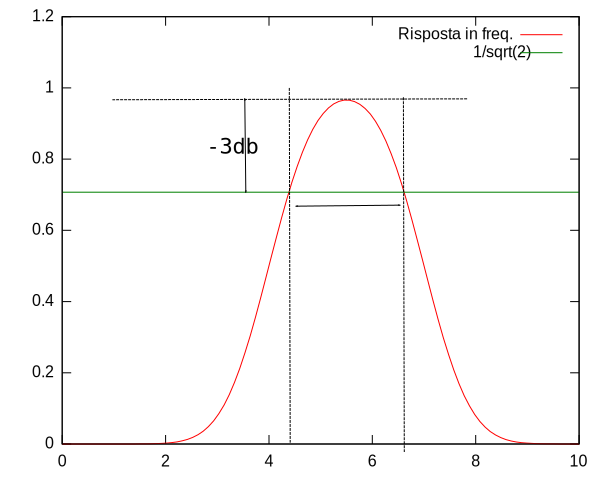
\includegraphics[width=0.6\textwidth]{\imagedir/bw}
		  \caption{Misurazione della larghezza di banda di un filtro\label{fig:bw}}
		\end{center}
	\end{figure}

	Quando un filtro ha un polo collocato da qualche parte sul piano $z$ questo
    polo avr\`a un modulo R e un angolo $\theta$.
  
	Consideriamo ora l'effetto di un polo sul cerchio unitario sull'asse reale:
    se $\theta$ \`e 0 avremo un filtro passa basso e l'algebra si semplifica. Se
    $\theta$ \`e non-zero l'effetto sar\`a uguale ruotato di un angolo
		$\theta$.
  
	Dato che per i fitri IIR a un polo la funzione di trasferimento \`e
  
		 \begin{equation}
				H(z) = \frac{1}{1 - a_1 z^{-1}}
		 \end{equation}

	l'inverso del quadrato della della risposta in magnitudine ad una frequenza
    $\psi (rad/campione)$ legata a questo polo sull'asse reale laddove $z = R$ \`e
  
		 \begin{equation}
				\frac{1}{|H(z)|^2} = |1 - a_1 z^{-1}|^2 = | z - a_1 |^2
		 \end{equation}
  
    ponendo $z = e^{i\theta}$ e $a_1 = R$
  
		 \begin{equation}
				\frac{1}{|H(z)|^2} =  |e^{i\theta} - R|^2
		 \end{equation}
  
    svolgendo il modulo
  
		 \begin{equation}
				\frac{1}{|H(z)|^2} =  1 - 2 R cos\,\theta + R^2
		 \end{equation}
  
	Nel centro della risonanza $\theta = 0$, $cos\,\theta = 1$ e l'equazione diventa:
  
		 \begin{equation}
				\frac{1}{|H(z)|^2} =  1 - 2 R cos\,\theta + R^2
		 \end{equation}

		 \begin{equation}
				\frac{1}{|H(z)|^2} =  1 - 2 R + R^2 = (1 - R)^2
		 \end{equation}

		cio\`e il quadrato della distanza tra
    la frequenza zero sul cerchio unitario $(z = 1)$ \`e il polo
  
  Per trovare i punti in cui la magnitudine \`e $1/\sqrt{2}$, guardiamo
    per quale $\theta$ la magnitudine \`e il doppio di questo, quindi:
  
		\begin{equation}\label{eqn:theta solution for bw}
    1 - 2 R cos \theta + R^2 = 2 (1 - R)^2 = 2 [ 1 - 2R + R^2 ]
		 \end{equation}
  
	Risolviamo quindi l'eq.\ref{eqn:theta solution for bw} per $\theta$:

	\begin{equation}
		- 2 R cos \theta = 2 - 4R + 2 R^2 - 1 - 2 R^2 = 1 - 4 R 
  \end{equation}

	ossia

	\begin{equation}
					cos \theta = -\frac{1}{2 R} + \frac{4 R}{2 R} = - \frac{1}{2R} + 2 R
  \end{equation}

	quindi

	\begin{equation}
		\theta = arccos \left ( 2 R  - \frac{1}{2 R} \right )
	\end{equation}

	%
	% VERIFICARE e inventare un PLOT che faccia vedere
	%
  
\section{Resons}
  
					I filtri a un polo hanno i poli e gli zeri che si dispongono
    soltanto a freq. zero o nyquist, a seconda del fatto che il polo sia pi\`u
    vicino a $z = +1$ o $z = -1$.
  
	Per avere filtri che risuonino ad una frequenza desiderata qualsiasi abbiamo
    (e per fare in modo che il filtro tiri fuori un segnale reale) ci vogliono
    almeno un paio di poli disposti in maniera complessa coniugata
  
		 \begin{equation}
						 H(z) = \frac{1}{(1 - Re^{i\theta} z^{-1})(1 - Re^{-i\theta} z^{-1})}
		 \end{equation}
  
    dove R \`e il modulo del polo e $\theta$ \`e l'angolo (frq) e $Re^{+/-\theta}$ sono le
    radici del denominatore (poli)
  
	Ora se eseguiamo la moltiplicazione del denominatore quello che otteniamo \`e:
  
		 \begin{equation}
			 \begin{array}{r c c c l c l}
     den & = & (1 & - & Re^{i\theta} z^{-1})(1 - Re^{-i\theta} z^{-1}) & &\\
         & = & 1 & - & Re^{-i\theta} z^{-1} - Re^{i\theta} z^{-1} & + & R^{2} z^{-2}\\
         & = & 1 & - & Rz^{-1} (e^{i\theta} + e^{-i\theta}) & + & R^{2} z^{-2}\\
         & = & 1 & - & Rz^{-1} 2 cos \theta & + & R^{2} z^{-2}\\
		 		\end{array}
		 \end{equation}
  
		 \begin{equation}
			 H(z) = \frac{1}{1 - (2R cos \theta) z^{-1} + R^{2} z^{-2}}
		 \end{equation}
  
   
	Se interpretiamo $z^{-1}$ come ``ritardo di un campione'', vediamo subito che
    questa funzione di trasferimento corrisponde al filtro:
  
		 \begin{equation}
    y_t = x_t + (2Rcos \theta) y_{t-1} - R^{2} y_{t-2}
		 \end{equation}
  
% \section{Determinazione della frequenza di un reson}
% 
%  	Per determinare la frequenza di risonanza del reson non si pu\`o prendere
%      direttamene $\theta$ perch\'e l'altro polo influenza la posizione del picco, e
%      quando i poli sono vicini lo shift \`e significativo
%    
%  	Adottiamo un approccio semplicistico: valutiamo la risposta in frequenza come funzione
%      della variabile di frequenza $\psi$ e poi troviamo la frequenza $\psi$ per cui la
%      derivata \`e zero. Per semplificare ulteriormente non prenderemo in
%      considerazione la magnitudine della frequenza, ma il quadrato del suo
%      inverso -- dato che la risposta in frequenza originale ha un massimo
% 		 proprio dove il quadrato del suo inverso ha un minimo
% 		 (cf.\vref{fig:inverse fr})
% 	\begin{figure}[htb]
% 		\begin{center}
% 			\includegraphics[width=0.6\textwidth]{\plotdir/inverse_fr}
% 			\caption{Inverso della risposta in frequenza per $\theta = \pi/15$ (confrontato col suo dritto)\label{fig:inverse fr}}
% 		\end{center}
% 	\end{figure}
% 
%    
%  	Riprendiamo il quadrato dell'inverso del modulo di $H(z)$:
%    
%  		 \begin{equation}
%      |(1 - Re^{i\theta} z^{-1})(1 - Re^{-i\theta} z^{-1})|^2
%  		 \end{equation}
%    
%    - questa volta conviene moltiplicare tutto per $z^2$ per ottenere la posizione dei
%      poli (dato che $z^2 = 1$ sul cerchio unitario, possiamo farlo)
%    
%  		 \begin{equation}
%      |(z - Re^{i\theta})(z - Re^{-i\theta})|^2
%  		 \end{equation}
%    
%    - sostituiamo $z = e^{i\theta}$
%    
%  		 \begin{equation}
%       |(e^{i\theta} - R e^{i\theta})(e^{i\theta} - Re^{-i\theta})|^2
%  		 \end{equation}
%    
%    % COMPLETARE

\section{Per migliorare i reson: aggiungere gli zeri}

Combinando \emph{feedback} (filtri a poli) con \emph{feed-forward} (filtri
FIR, con zeri) si migliora sostanzialmente la risposta dei filtri Reson
(ed è così che sono fatti normalmente). Questo permette di avere delle buone
risposte anche quando la campana del filtro \`e a bassa frequenza.

Un modo per migliorare la forma \`e quello di porre uno zero a $z = 1$, e
gi\`a che ci siamo per simmetria porne uno anche per $z = nyquist = \pi$.

Possiamo farlo moltiplicando la funzione di trasferimento del reson per un
fattore $1 - z^{-2}$, che pone degli zeri a $z = \pm 1$. Quindi la
funzione di trasferimento diventer\`a:

\begin{equation}
	H(z) = \frac{1 - z^{-2}}{1 - 2 R cos \theta z^{-1} + R^2 z^{-2}}
\end{equation}

\section{Filtri bi-quad (ellittici)}

Nei filtri FIR \`e sufficiente creare un numero esteso di termini (i.e. un
sufficiente numero di zeri) per ottenere la funzione di trasferimento
desiderata. La cosa \`e molto pi\`u complicata con i filtri IIR,
perch\'e i
poli sono pi\`u complicati da gestire che gli zeri.

Negli anni '30 i matematici hanno formulato alcune possibili risposte
``prefabbricate'' al problema. Una di queste, ad esempio, \`e il filtro
biquadratico (\emph{biquad}) \emph{ellittico}, il quale \`e combinabile in
serie e/o in parallelo per ottenere la funzione di trasferimento desiderata.
La forma canonica del filtro ellittico \`e

\begin{equation}
	H ( z ) = \frac{1 + a z^{-1} + b z^{-2}}{1 + c z^{-1} + d z^{-2}}	
\end{equation}

(due poli e due zeri).
Utilizzando questa forma in stadi successivi (filtri a cascata) \`e possibile
approssimare la funzione di trasferimento desiderata.
%
% provare ad utilizzare questi filtri in forma ``euristica'', usando ci\`o che
% abbiamo imparato dai filtri reson (applicando la formula del reson sopra e
% sotto per ottenere dei poli e zeri 


%
% $Id: comb.tex 14 2014-02-04 22:36:30Z nicb $
%
\svnInfo $Id: comb.tex 14 2014-02-04 22:36:30Z nicb $

\chapter{Filtri a pettine (Comb)\label{chap:comb}}

Quando abbiamo studiato i filtri FIR (cf. Cap.\ref{chap:fir}) abbiamo
visto che si possono realizzare filtri nella forma

\begin{equation}\label{eq:invcomb}
  y_t = x_t - R^{L} x_{t-L}
\end{equation}

dove $y$ e $x$ sono, come di consueto, rispettivamente la nostra uscita e il
nostro ingresso. Questi filtri erano costituiti dalla somma algebrica
dell'ingresso e della sua copia ritardata di $L$ campioni.

Se sostituiamo all'ingresso ritardato \emph{l'uscita} ritardata, otteniamo

\begin{equation}
  y_t = x_t + R^{L} y_{t-L}
\end{equation}

La rappresentazione vettoriale di questa equazione \`e

\begin{equation}
  Y = X + R^{L} z^{-L} Y
\end{equation}

Se raggruppo i fattori ottengo

\begin{equation}
  Y - R^{L} z^{-L} Y = Y ( 1 - R^{L} z^{-L} ) = X
\end{equation}

ossia

\begin{equation}
  Y = \frac{X}{1 - R^{L} z^{-L}}
\end{equation}

Quindi la funzione di trasferimento \`e

\begin{equation}
 H ( z ) = \frac{1}{1 - R^{L} z^{-L}}
\end{equation}

Un filtro con questa funzione di trasferimento si chiama
\emph{filtro a pettine}.

Questa funzione di trasferimento \`e il reciproco della funzione di
trasferimento dell'equazione \ref{eq:invcomb}. Quindi se li mettiamo in 
cascata otteniamo una risposta unitaria perch\'e l'azione del primo
canceller\`a quella del secondo.
Per constatare questo basta metterli uno dietro l'altro:

\begin{equation}
  \begin{array}{r c r c l}
	  y_t & = & x_t & - & R^{L} x_{t-L}\\
		w_t & = & y_t & + & R^{L} w_{t-L}\\
	\end{array}
\end{equation}

($w_t$ \`e l'uscita ottenuta usando l'uscita del primo filtro, $y_t$, come
ingresso del secondo filtro).

Ma

\begin{equation}
  y_t = w_t - R^{L} w_{t-L}
\end{equation}

Se sostituisco $y_t$ nella prima equazione ottengo

\begin{equation}
	x_t - R^{L} x_{t-L} = w_t - R^{L} w_{t-L}
\end{equation}

Se il segnale \`e causale, noteremo che $x_t = w_t$
per $t = 0, 1, \dots , L - 1$ dato che $x_{t - L}$ e $w_{t - L}$
valgono zero in quell'ambito.
Applicando lo stesso ragionamento potremo osservare che
$x_t = w_t$ per $t = L, L + 1, \dots, 2 L - 1$. E cos\`i via a blocchi di $L$
campioni. Quindi evidentemente si tratta dello stesso segnale spostato di $L$
campioni.

\begin{figure}[htbp]
	\begin{center}
	\includegraphics[width=0.75\textwidth]{\plotdir/comb_2}
	\caption{La collocazione dei poli in un filtro comb di ottavo ordine con
	fattore $R = 0.999999$\label{fig:comb poles}}
	\end{center}
\end{figure}

\begin{figure}[htbp]
	\begin{center}
	\includegraphics[width=0.75\textwidth]{\plotdir/comb_1}
	\caption{Magnitudine e fase di un filtro comb di ottavo ordine con
	fattore $R = 0.999999$\label{fig:comb magnitude and phase}}
	\end{center}
\end{figure}

\begin{figure}[htbp]
	\begin{center}
	\includegraphics[width=0.75\textwidth]{\plotdir/comb_3}
	\caption{Magnitudine di un filtro comb di ottavo ordine con
	fattore $R = 0.999999$ sul piano zeta\label{fig:comb z-plane poles}}
	\end{center}
\end{figure}

\section{Implementazione \emph{real--world}}

Nel mondo reale i filtri a pettine vengono usati per diversi effetti in campo
audio e musicale. La fig.\vref{fig: real world comb} illustra la risposta
all'impulso di un filtro comb con frequenza di risonanza $233 Hz$, ossia con
un ritardo di 189 campioni.
\begin{figure}[htbp]
	\begin{center}
	  \includegraphics[width=0.75\textwidth]{\plotdir/comb_real}
	  \caption{Risposta all'impulso di un filtro a pettine con frequenza di
		risonanza $233 Hz$\label{fig: real world comb}}
	\end{center}
\end{figure}

\section{Analogia con le onde stazionarie}

Riflettendoci sopra, i filtri comb altro non fanno che aggiungere l'uscita
attenuata e ritadata di $L$ campioni all'ingresso. E` il meccanismo
dell'\emph{eco}.

C'\`e anche una robusta analogia con la riflessione delle onde stazionarie,
ad esempio in un tubo con entrambi le estremit\`a chiuse (o con entrambi le
estremit\`a aperte): le estremit\`a chiuse cambiano di segno alla riflessione
mentre le estremit\`a aperte no. Le altre onde che si propagano in questo modo
sono quelle delle corde tenute ferme ad entrambe le estremit\`a.


%
% $Id: karplus_strong.tex 14 2014-02-04 22:36:30Z nicb $
%
\svnInfo $Id: karplus_strong.tex 14 2014-02-04 22:36:30Z nicb $

\chapter{Filtri delle corde pizzicate}

Cosa succede se immetto un impulso unitario in un filtro comb?
Semplicemente, l'impulso torner\`a $L$ campioni dopo moltiplicato per il
coefficiente $R^L$.

Tutti gli altri campioni valgono $0$, per cui non succede niente tra il tempo
$0$ e il tempo $L$.

La risposta all'impulso sar\`a quindi:

% \begin{equation}
% 	h_t = \left \{ \begin{array}{l l l}
% 			R^t & & se t = 0 mod L\\
% 			0   & & per tutti gli altri campioni\\
% 	 \end{array}
% \end{equation}

Ossia $h_t = R^t$ per $t = 0,~L,~2L, \dots$ e $0$ altrimenti. Questa \`e una
sequenza periodica di impulsi alla frequenza fondamentale di $f_c / L~Hz$ -- una
frazione intera della frequenza di campionamento,
salvo il fatto che questi impulsi decadono con una velocit\`a determinata da $R$.
Pi\`u $R$ \`e vicino a 1, pi\`u lento sar\`a il decadimento, e viceversa.

Fin qui, nulla di particolarmente eccitante.
I suoni musicali, in particolare quelli percussivi,
sono caratterizzati da una variazione dello spettro nel tempo.
E` vero che in questo caso il suono decade nel tempo, ma il suo spettro
\emph{decade tutto insieme} e quindi non si modifica in maniera musicale.

Karplus e Strong suggerirono una modifica del filtro comb per poterlo rendere pi\`u musicale.
L'idea \`e semplicissima: si tratta di inserire un filtro passa--basso nel
loop di feedback in modo da attenuare pi\`u rapidamente le frequenze acute
rispetto a quelle gravi.

Il filtro passabasso pu\`o anche essere un semplicissimo filtro di media

\begin{equation}
				y_t = \nicefrac{1}{2} \left [ x_t + x_{t-1} \right ]
\end{equation}

con funzione di trasferimento

\begin{equation}\label{eqn: ks lop transfer function}
				H (z) = \nicefrac{1}{2} \left [ 1 + z^{-1} \right ]
\end{equation}

con uno zero che si trova in corrispondenza della frequenza di Nyquist,
poich\'e l\`i $z = -1$.
% Sostituendo $z = e^{i\omega}$ nell'eq.\ref{eqn: ks lop transfer function} avremo che
% 
% \begin{equation}\label{eqn: ks lop transfer function unit circle}
% 				H (\omega) = \nicefrac{1}{2} \left [ 1 + e^{-i\omega} \right ] = \nicefrac{1}{2} + \nicefrac{1}{2} e^{-i\omega}
% \end{equation}

\begin{figure}[htbp]
	\begin{center}
		\includegraphics[width=0.75\textwidth]{\plotdir/ks_lop}
		\caption{La risposta in frequenza del filtro passabasso usato
		nell'algoritmo di Karplus e Strong\label{fig:ks lop frequency response}}
	\end{center}
\end{figure}

\section{Implementazione dei filtri delle corde pizzicate}

Per scrivere l'equazione del filtro,
\`e utile introdurre il segnale intermedio $w$,
il quale compare immedatamente dopo la chiusura del loop di feedback.
Il segnale $w$ \`e quindi determinato dall'ingresso $x$ e dal segnale di
output ritardato e pesato $y$:

\begin{equation}\label{eqn: ks first part}
				w_t = x_t + R^{L} y_{t-L}
\end{equation}

mentre l'uscita al tempo $t$ \`e determinata dal filtro FIR con input $w$,
quindi

\begin{equation}\label{eqn: ks second part}
				y_t = \nicefrac{1}{2} w_t + \nicefrac{1}{2} w_{t - 1}
\end{equation}

Quindi per ogni campione $t$ dobbiamo prima trovare $w_t$ nei termini
dell'equazione \ref{eqn: ks first part} e poi il valore dell'uscita $y_t$ da
$w_t$ e $w_{t - 1}$ secondo l'equazione \ref{eqn: ks second part}.

Cerchiamo ora di capire quale sia la risposta in frequenza di questo filtro.
Se guardiamo il segnale come vettore, le equazioni \ref{eqn: ks first part} e
\ref{eqn: ks second part} diventano

\begin{equation}\label{eqn: ks 1 ztransf}
		W = X + R^{L} z^{-L} Y
\end{equation}

\begin{equation}\label{eqn: ks 2 ztransf}
		Y = \nicefrac{1}{2} [ 1 + z^{-1} ] W
\end{equation}

Per trovare la funzione di trasferimento $H(z)$ dobbiamo risolvere l'equazione
per $Y / X$, ossia prima sostituire l'eq.\ref{eqn: ks 1 ztransf}
nell'eq.\ref{eqn: ks 2 ztransf} per ottenere solo $X$ e $Y$

\begin{equation}\label{eqn: ks X}
				X = 1 - R^L z^{-L} \nicefrac{1}{2} [ 1 + z^{-1} ]  
\end{equation}

e da qui trovare la funzione di trasferimento

\begin{equation}\label{eqn: ks transfer function}
				H ( z ) = Y / X = \frac{\nicefrac{1}{2} [ 1 + z^{-1} ]}{1 - R^{L} z^{-L} \nicefrac{1}{2} [ 1 + z^{-1} ]}
\end{equation}

Per risolvere questa equazione dobbiamo prima ottenere una formula pi\`u
chiara. Possiamo moltplicare numeratore e denominatore per $2 z^{L + 1}$:

\begin{equation}\label{eqn: ks transfer function 2}
				H ( z ) = Y / X = \frac{\nicefrac{1}{2} [ 1 + z^{-1} ] 2 z^{L+1}}{(1 - R^{L} z^{-L} \nicefrac{1}{2} [ 1 + z^{-1} ]) 2 z^{L + 1}} = \frac{z^{L + 1} + z^{L}}{2 z^{L+1} - R^{L} z - R^{L}}
\end{equation}

Per avere la risposta in frequenza dobbiamo valutare l'eq.\ref{eqn: ks transfer function 2}
sul cerchio unitario, quindi quando $z = e^{i \omega}$. Possiamo quindi
sostituire $z$ usando la formula di Eulero:

\begin{equation}
	\begin{array}{r c l}
		z & = & cos \omega + i sen \omega\\
		z^{L} & = & cos ( L \omega ) + i sen ( L \omega )\\
		z^{L+1} & = & cos ( (L + 1) \omega ) + i sen ( (L + 1) \omega )\\
	\end{array}
\end{equation}

Separando quindi le parti reali e le parti immaginarie dell'eq.\ref{eqn: ks
transfer function 2} sia al numeratore che al denominatore ottengo:

\begin{equation}\label{eqn: ks transfer function separated}
	\begin{array}{r c l}
		Reale ( numeratore ) & = & cos ( ( L + 1 ) \omega ) + cos ( L \omega )\\
		Immag ( numeratore ) & = & sin ( ( L + 1 ) \omega ) + sin ( L \omega )\\
		Reale ( denominatore ) & = & 2 cos ( ( L + 1 ) \omega ) - R^{L} cos \omega - R^{L} )\\
		Immag ( denominatore ) & = & 2 sin ( ( L + 1 ) \omega ) - R^{L} sin \omega )\\
	\end{array}
\end{equation}

A questo punto per trovare la risposta in frequenza devo trovare la
magnitudine di $H(z)$ sostituendo le equazioni \ref{eqn: ks transfer function separated}:

\begin{equation}\label{eqn: ks magnitude response}
				| H ( \omega ) | = \left [ \frac{[ Reale (numeratore) ]^{2} + [ Immag (numeratore) ]^{2}}{[ Reale (denominatore) ]^{2} + [ Immag (denominatore) ]^{2}} \right ]^{1/2}
\end{equation}

Realizziamone un'implementazione concreta per $L = 32$ con un coefficiente $R = 0.999$.
Dato che il ritardo totale del loop di feedback sar\`a di $32.5$ campioni,
ci aspettiamo che le risonanze siano ai multipli di $f_c / 32.5$.


\bibliographystyle{apalike}
\bibliography{\dirroot/CSEDSM}

\end{document}
